\subsection{ArbIS}
\label{analysis_processing_correlation_arbis_matched}
As with the congestion - accident datasets in \cref{analysis_processing_correlation_baysis_matched,analysis_processing_correlation_baysis_initiator,analysis_processing_correlation_baysis_effector,analysis_processing_correlation_baysis_follower} the congestion - roadwork dataset also needs to be analyzed for correlations. The correlation matrix table for the congestion-roadwork dataset (see \cref{tbl:appendix_arbis_correlation_matrix_dataset_cramers}) is visual presented in \cref{img:correlation_matrix_arbis_selected_effector_cramers} showing the the correlation of each variable combination. When visual analyzing \cref{img:correlation_matrix_arbis_selected_effector_cramers} and checking the guidelines for a strong correlation in reference to the applied coefficient (identifiable with \cref{table:appendix_coefficient_matrix_matched}) we get a list of strongly correlated variable combinations (see \cref{tbl:correlation_list_arbis_matched}). Since the focus of the thesis are the correlations between accidents and jams, these are only collected from the bottom-left rectangle of the matrix, where the congestion and accidents variables intersect. Correlations of the kind congestion - congestion or roadwork - roadwork are not considered.
\begin{table}[h!]
	\centering
	\begin{tabular}{c|l|l}  
		Category & Strong \\
		\\[-1em]
		\hline
		\\[-1em]
		Strasse & TMax, TAvg, SMax, SAvg, TDist, SDist, Cov, TLCar, TLHGV \\ 
 		%AnzGesperrtFs & & \\ 
 		%Einzug & & \\
 		%Richtung & & \\
 		%Length & & \\
 		%Duration & & \\
 		Month & TAvg, SMax, SAvg, TDist, SDist, Cov, TLCar \\
	\end{tabular}
  \caption{List of incident variables and their strong/moderated correlated jam variable from the ArbIS matched data}
  \label{tbl:correlation_list_arbis_matched}
\end{table}
As \cref{tbl:correlation_list_arbis_matched} show, only the variables Strasse and Month are correlated with congestion characteristics. Both variables tend to bias an interpretation of congestion characteristics because the 


Next we need to verify that the correlation is significant and what the correlation predicates. Therefore each correlation will be evaluated with the Post Hoc test, defined in \cref{correlation_posthoc}. In the following sections, the correlated relations of the variables in \cref{tbl:correlation_list_arbis_matched} are analyzed and an initial interpretation of each significant correlation is introduced. Groups with an insufficient sample size (see \cref{correlation_uncertainty} are neglected and not shown. The descriptive tables, showing the count ($n$), mean ($\bar{x}$), standard deviation ($\sigma$), median ($\tilde{x}$), $min$, $max$ and range ($\Delta$) therefore only contain groups with significant sample sizes.
\begin{figure}[!ht]
	\centering
	\makebox[\textwidth][c]{%
		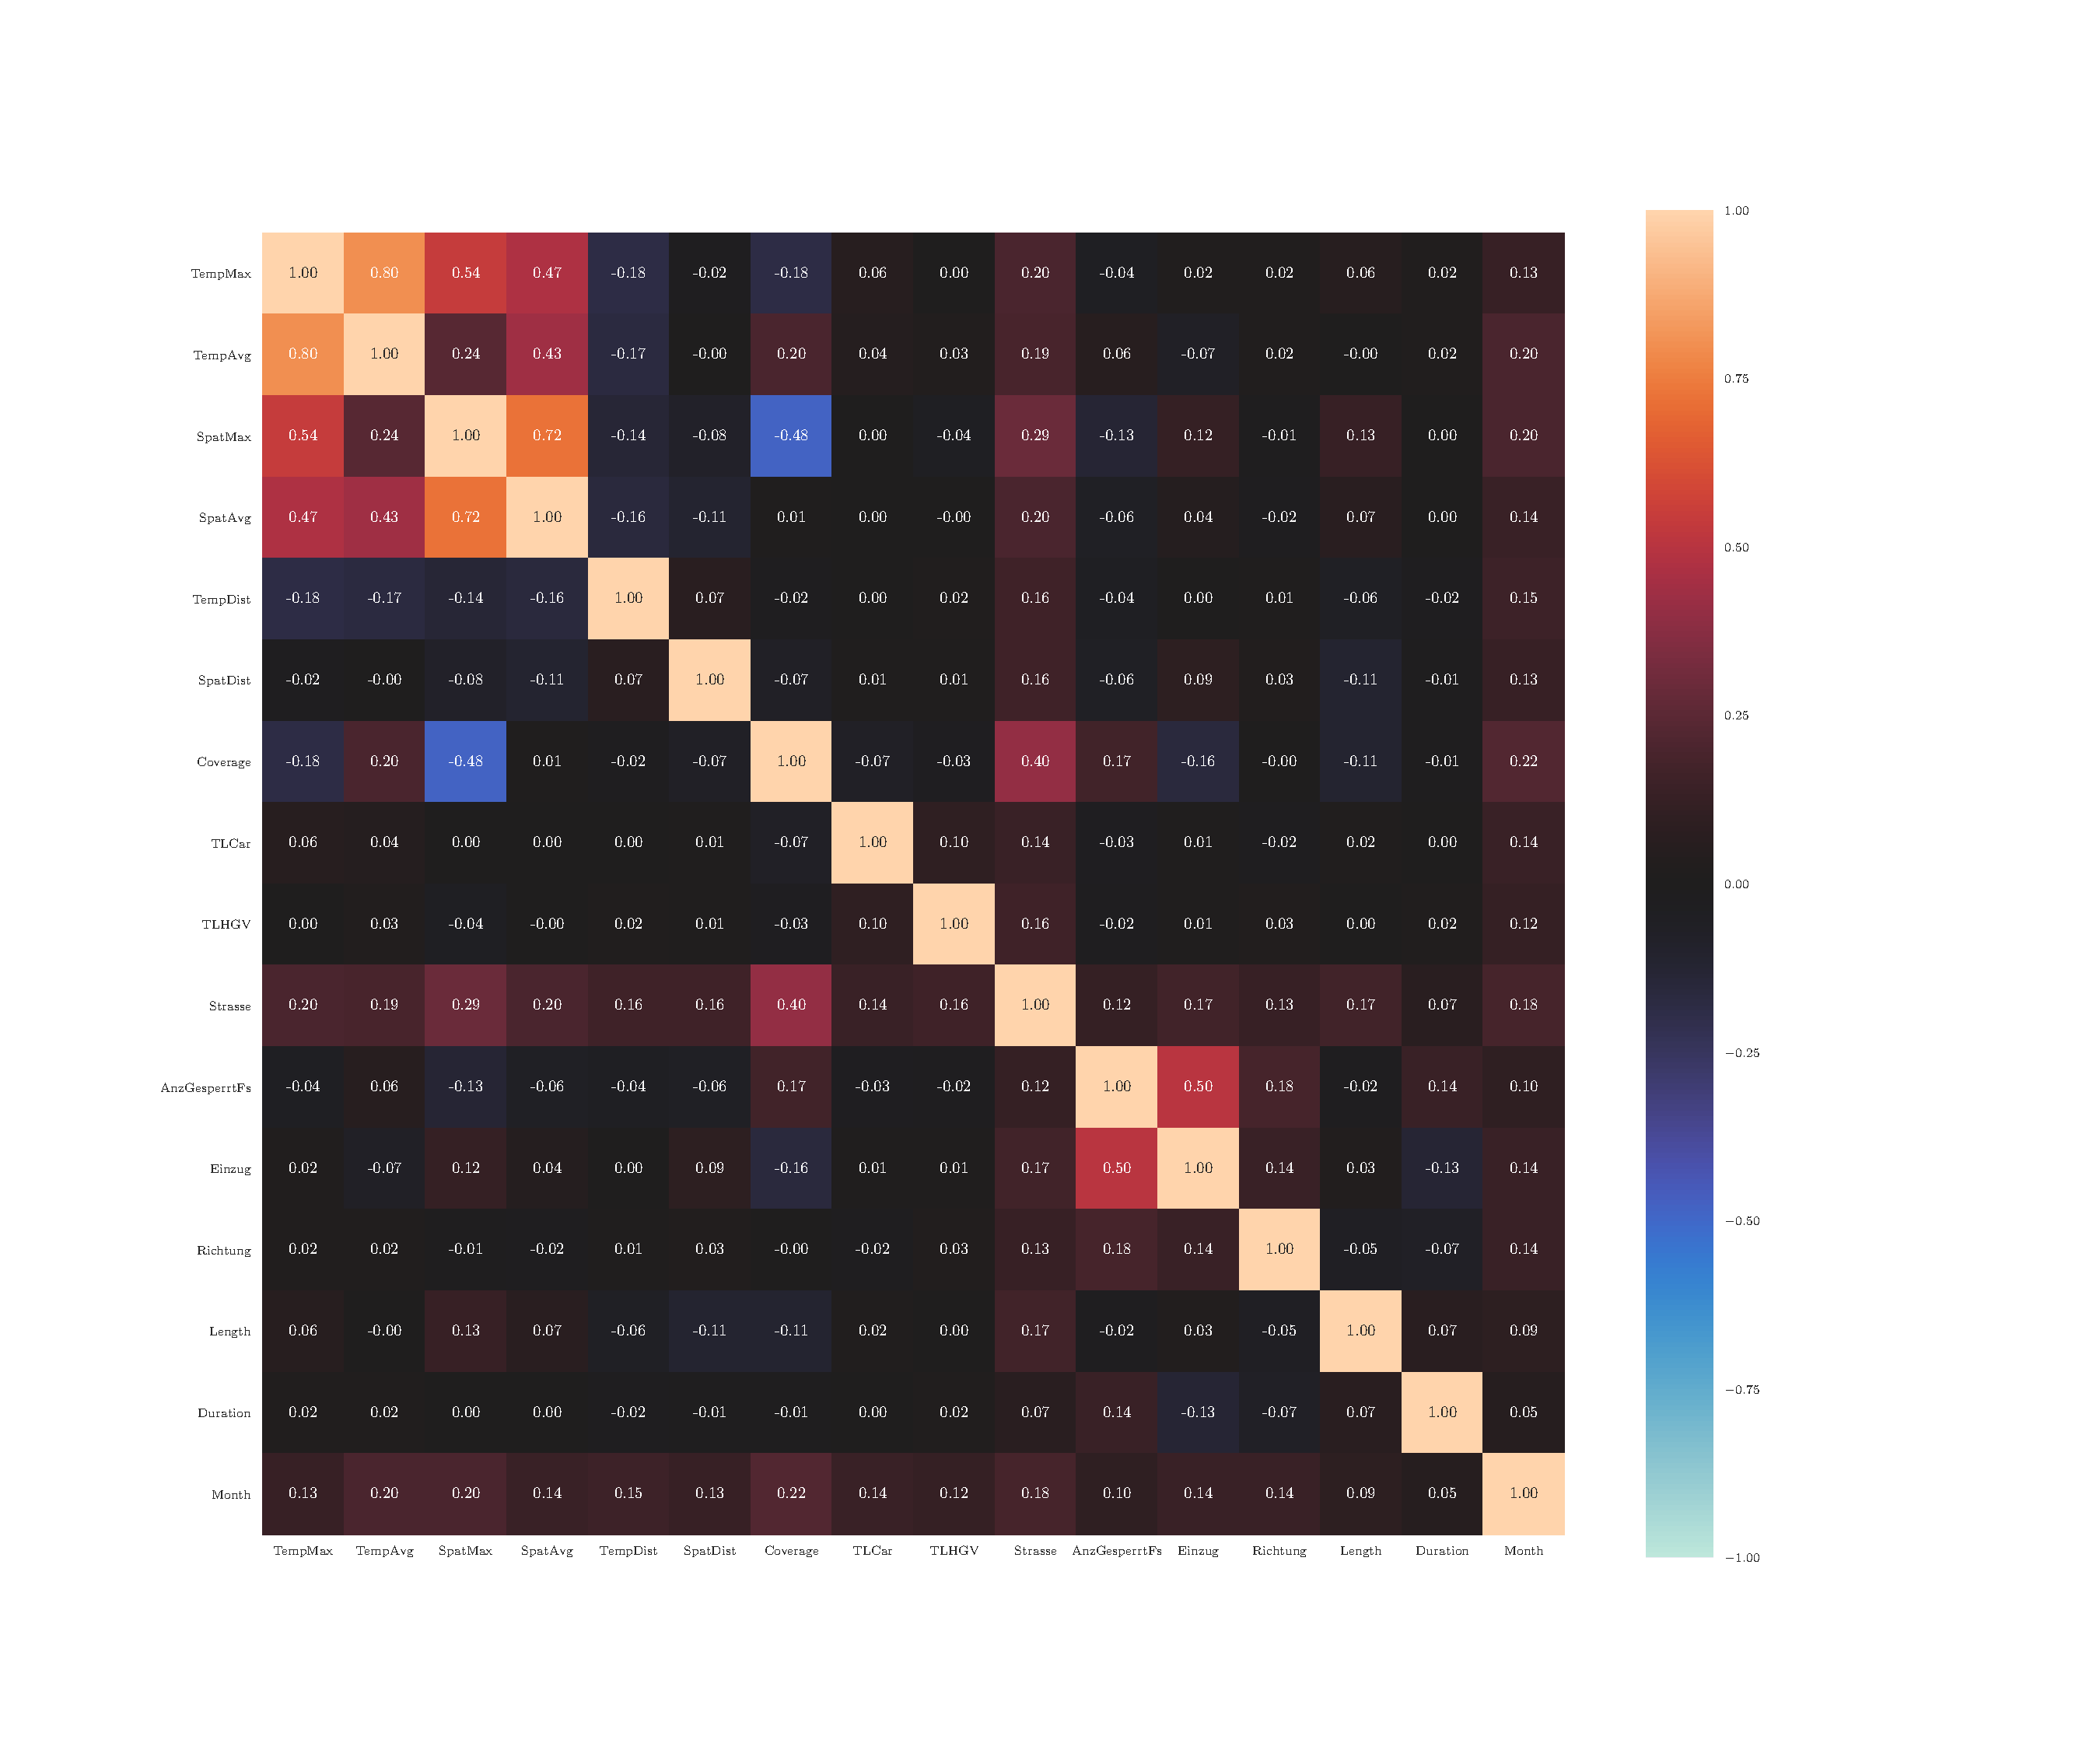
\includegraphics[width=1.4\textwidth, trim=0cm 2.5cm 6cm 3cm]{CorrAnalysis/data/ArbIS/02_matched/plots/arbis_matched_corr_cramers}%
	}
	\caption{Correlation matrix for congestion-roadwork matched data, calculated with $V$, $\eta$, $\tau$, $r_{pq}$, $r$}
	\label{img:correlation_matrix_arbis_selected_effector_cramers}
\end{figure}

% % --------------------------
% % -------- Strasse ---------
% % --------------------------
\centerheading{Strasse}
This section analyzes the correlated relations of the accident variable \textit{Strasse}. The Kruskal-Wallis rank sum test of \textit{Strasse} - \textit{TMax} produces a $p$-value of < 0.0001, which is below $\alpha$. The null hypothesis can therefore be rejected, which means there is a significant difference between the groups of \textit{Strasse}. To identify the significant groups, a pairwise Wilcoxon $T$-test for \textit{Strasse} - \textit{TMax} is run, which produces \cref{tbl:wilcoxon_arbis_matched_Strasse_TMax}. 
\begin{table}[ht!]
	\tiny
	\centering
    \begin{tabular}{rrrrrrrrrrrrrrrrr}
		\toprule
			& A9 & A7 & A70 & A71 & A6 & A73 & A3 & A99 & A96 & A995 & A92 & A72 & A93 & A95 & A94 & A980 \\ 
		\midrule
		% A7   & 1.00 &  &  &  &  &  &  &  &  &  &  &  &  &  &  &  \\ 
		% A70  & 1.00 & 1.00 &  &  &  &  &  &  &  &  &  &  &  &  &  &  \\ 
		% A71  & 1.00 & 1.00 & 1.00 &  &  &  &  &  &  &  &  &  &  &  &  &  \\ 
		% A6   & 1.00 & 1.00 & 1.00 & 1.00 &  &  &  &  &  &  &  &  &  &  &  &  \\ 
		% A73  & 1.00 & 1.00 & 1.00 & 1.00 & 1.00 &  &  &  &  &  &  &  &  &  &  &  \\ 
		A3   & \red{0.00} & \red{0.04} & 1.00 & 1.00 & \red{0.01} & 1.00 &  &  &  &  &  &  &  &  &  &  \\ 
		% A99  & 1.00 & 1.00 & 1.00 & 1.00 & 0.48 & 1.00 & 1.00 &  &  &  &  &  &  &  &  &  \\ 
		A96  & 1.00 & 0.82 & 1.00 & 1.00 & 1.00 & 1.00 & \red{0.00} & \red{0.00} &  &  &  &  &  &  &  &  \\ 
		% A995 & 1.00 & 1.00 & 1.00 & 1.00 & 1.00 & 1.00 & 0.79 & 0.74 & 1.00 &  &  &  &  &  &  &  \\ 
		% A92  & 1.00 & 1.00 & 1.00 & 1.00 & 1.00 & 1.00 & 1.00 & 1.00 & 1.00 & 1.00 &  &  &  &  &  &  \\ 
		% A72  & 1.00 & 1.00 & 1.00 & 1.00 & 1.00 & 1.00 & 1.00 & 1.00 & 1.00 & 1.00 & 1.00 &  &  &  &  &  \\ 
		A93  & \red{0.00} & \red{0.00} & 1.00 & 0.09 & \red{0.00} & \red{0.00} & 1.00 & 1.00 & \red{0.00} & \red{0.00} & \red{0.00} & 1.00 &  &  &  &  \\ 
		% A95  & 1.00 & 1.00 & 1.00 & 1.00 & 1.00 & 1.00 & 1.00 & 1.00 & 1.00 & 1.00 & 1.00 & 1.00 & 1.00 &  &  &  \\ 
		A94  & 1.00 & 1.00 & 1.00 & 1.00 & 0.68 & 1.00 & 1.00 & 1.00 & \red{0.01} & 0.48 & 1.00 & 1.00 & 1.00 & 1.00 &  &  \\ 
		% A980 & 1.00 & 1.00 & 1.00 & 1.00 & 1.00 & 1.00 & 1.00 & 1.00 & 1.00 & 1.00 & 1.00 & 1.00 & 1.00 & 1.00 & 1.00 &  \\ 
		% A45  & 1.00 & 1.00 & 1.00 & 1.00 & 1.00 & 1.00 & 1.00 & 1.00 & 1.00 & 1.00 & 1.00 & 1.00 & 1.00 & 1.00 & 1.00 & 1.00 \\ 
		\bottomrule
	\end{tabular}
	\caption{Pairwise Wilcoxon $T$-test for \textit{Strasse} and \textit{Maximal Temporal Extent}}
	\label{tbl:wilcoxon_arbis_matched_Strasse_TMax}
\end{table}
The table shows, that the groups A3 and A93 differ from group A9, A7 and A6. The A93 also differs from A96, A995 and A92. The A96 differs from A3 and A99.
\pgfplotstableread[col sep=comma,header=false]{
	A9   , 656  , 159.55 , 175.78 , 100.50 , 9   , 1323 , 1314
	A7   , 302  , 158.38 , 213.55 , 87.00  , 9   , 1323 , 1314
	A70  , 50   , 228.90 , 279.03 , 105.00 , 15  , 963  , 948 
	A71  , 10   , 83.40  , 72.87  , 48.00  , 36  , 249  , 213 
	A6   , 198  , 142.24 , 166.46 , 85.50  , 9   , 864  , 855 
	A73  , 86   , 153.59 , 235.85 , 100.50 , 9   , 1323 , 1314
	A3   , 1023 , 233.66 , 279.35 , 123.00 , 9   , 1326 , 1317
	A99  , 312  , 158.88 , 155.05 , 135.00 , 9   , 1320 , 1311
	A96  , 230  , 105.80 , 95.17  , 75.00  , 9   , 384  , 375 
	A995 , 14   , 60.00  , 28.70  , 48.00  , 18  , 105  , 87 
	A92  , 82   , 132.40 , 134.72 , 79.50  , 9   , 768  , 759 
	A93  , 160  , 157.33 , 55.97  , 189.00 , 9   , 312  , 303 
	A94  , 56   , 179.57 , 124.79 , 165.00 , 15  , 369  , 354 
}\data
\pgfplotstablecreatecol[
  create col/expr={\thisrow{1} + \thisrow{2} + \thisrow{3} + \thisrow{4}}
]{sum}{\data}
\begin{figure}[ht!]
	\centering
	\begin{minipage}{0.5\textwidth}
		\tiny
		\centering
		\begin{tabular}{c|c|c|c|c|c|c|c}
			\toprule
			Group & $n$ & $\bar{x}$ & $\sigma$ & $\tilde{x}$ & $min$ & $max$ & $\Delta$ \\
			\midrule
			A9   & 656  & 159.55 & 175.78 & 100.50 & 9   & 1323 & 1314 \\ 
			A7   & 302  & 158.38 & 213.55 & 87.00  & 9   & 1323 & 1314 \\ 
			A70  & 50   & 228.90 & 279.03 & 105.00 & 15  & 963  & 948 \\ 
			A71  & 10   & 83.40  & 72.87  & 48.00  & 36  & 249  & 213 \\ 
			A6   & 198  & 142.24 & 166.46 & 85.50  & 9   & 864  & 855 \\ 
			A73  & 86   & 153.59 & 235.85 & 100.50 & 9   & 1323 & 1314 \\ 
			A3   & 1023 & 233.66 & 279.35 & 123.00 & 9   & 1326 & 1317 \\ 
			A99  & 312  & 158.88 & 155.05 & 135.00 & 9   & 1320 & 1311 \\ 
			A96  & 230  & 105.80 & 95.17  & 75.00  & 9   & 384  & 375 \\ 
			A995 & 14   & 60.00  & 28.70  & 48.00  & 18  & 105  & 87 \\ 
			A92  & 82   & 132.40 & 134.72 & 79.50  & 9   & 768  & 759 \\ 
			A93  & 160  & 157.33 & 55.97  & 189.00 & 9   & 312  & 303 \\  
			A94  & 56   & 179.57 & 124.79 & 165.00 & 15  & 369  & 354 \\ 
			\bottomrule
			% \bar{x} - sum = 1953,7, mean = 150.28
			% \sigma - sum = 2017.29, mean = 155,17
		\end{tabular}
		\subcaption[second caption.]{Table of all descriptives}\label{tbl:descriptives_arbis_matched_Strasse_TMax}
	\end{minipage}%
	\begin{minipage}{0.5\textwidth}
		\tiny
		\centering
		% https://texwelt.de/fragen/26286/zwei-gruppen-bei-einem-gestapelten-balkendiagramm-und-zentrierte-balkenbeschriftungen
		% https://tex.stackexchange.com/questions/275229/forcing-all-axis-labels-to-display-in-a-plot
		\begin{tikzpicture}
			\begin{axis}[
				% Gitterlinien für y-Ticks
				width=\textwidth,
				height=5.5cm,
				xmajorgrids=true,
				ymajorgrids=true,
				xtick=data,
				xmin=0.5,
				% xticklabels={A9,A7,A70,A71,A6,A73,A3,A99,A96,A995,A92,A93,A94},
				xticklabels from table={\data}{[index]0},
				% zusätzliche Beschriftung an y-Achse
				every extra y tick/.style={
					tick0/.initial=blue,
					tick1/.initial=red,
					yticklabel style={
						color=\pgfkeysvalueof{/pgfplots/tick\ticknum}
					},
				},
				extra y ticks={150,155},
			]
			\addplot table [absolute series=2] {\data};
			\addplot table [absolute series=3] {\data};
			\addplot table [absolute series=4] {\data};
			\legend{
				$\bar{x}$,$\sigma$,$\tilde{x}$}
			\end{axis}
		 \end{tikzpicture}\vfill
		\subcaption[second caption.]{Plot of descriptives $\bar{x}$, $\sigma$ and $\tilde{x}$}\label{fig:descriptives_arbis_matched_Strasse_TMax}
	\end{minipage}%
	\caption{Group descriptives of \textit{Strasse} and \textit{Maximal Temporal Extent}}
	%\vspace{-8mm}
\end{figure}
With the descriptives in \cref{tbl:descriptives_arbis_matched_Strasse_TMax} and the named significant differences it can be interpreted that roadworks on the A3 result in 80\,\% longer $\bar{x}$ than on the A9, A7 and A6. The A70 has a similar difference. Roadworks on the A96 and A995 result in significantly shorter $\bar{x}$ than on the A3 and A99.

The Kruskal-Wallis rank sum test of \textit{Strasse} - \textit{TAvg} produces a $p$-value of < 0.0001, which is below $\alpha$. The null hypothesis can therefore be rejected, which means there is a significant difference between the groups of \textit{Strasse}. To identify the significant groups, a pairwise Wilcoxon $T$-test for \textit{Strasse} - \textit{TAvg} is run, which produces \cref{tbl:wilcoxon_arbis_matched_Strasse_TAvg}. 
\begin{table}[ht!]
	\tiny
	\setlength{\tabcolsep}{4pt}
	\centering
	\begin{tabular}{rrrrrrrrrrrrrrrrr}
		\toprule
			& A9 & A7 & A70 & A71 & A6 & A73 & A3 & A99 & A96 & A995 & A92 & A72 & A93 & A95 & A94 & A980 \\ 
		\midrule
		% A7   & 1.00 &  &  &  &  &  &  &  &  &  &  &  &  &  &  &  \\ 
		% A70  & 1.00 & 1.00 &  &  &  &  &  &  &  &  &  &  &  &  &  &  \\ 
		% A71  & 1.00 & 1.00 & 1.00 &  &  &  &  &  &  &  &  &  &  &  &  &  \\ 
		% A6   & 1.00 & 1.00 & 1.00 & 1.00 &  &  &  &  &  &  &  &  &  &  &  &  \\ 
		% A73  & 1.00 & 1.00 & 1.00 & 1.00 & 1.00 &  &  &  &  &  &  &  &  &  &  &  \\ 
		% A3   & 1.00 & 1.00 & 1.00 & 1.00 & 0.69 & 1.00 &  &  &  &  &  &  &  &  &  &  \\ 
		A99  & \red{0.00} & \red{0.00} & 0.08 & 1.00 & 1.00 & 1.00 & \red{0.00} &  &  &  &  &  &  &  &  &  \\ 
		% A96  & 1.00 & 1.00 & 1.00 & 1.00 & 1.00 & 1.00 & 1.00 & 0.55 &  &  &  &  &  &  &  &  \\ 
		% A995 & 1.00 & 1.00 & 1.00 & 1.00 & 1.00 & 1.00 & 1.00 & 1.00 & 1.00 &  &  &  &  &  &  &  \\ 
		A92  & 1.00 & 1.00 & 1.00 & 1.00 & 1.00 & 1.00 & 1.00 & \red{0.04} & 1.00 & 1.00 &  &  &  &  &  &  \\ 
		% A72  & 1.00 & 1.00 & 1.00 & 1.00 & 1.00 & 1.00 & 1.00 & 1.00 & 1.00 & 1.00 & 1.00 &  &  &  &  &  \\ 
		A93  & \red{0.00} & \red{0.00} & 1.00 & 0.24 & \red{0.00} & \red{0.00} & \red{0.00} & \red{0.00} & \red{0.00} & \red{0.00} & \red{0.00} & 1.00 &  &  &  &  \\ 
		% A95  & 1.00 & 1.00 & 1.00 & 1.00 & 1.00 & 1.00 & 1.00 & 1.00 & 1.00 & 1.00 & 1.00 & 1.00 & 1.00 &  &  &  \\ 
		A94  & 1.00 & 1.00 & 1.00 & 1.00 & 0.14 & 1.00 & 1.00 & \red{0.00} & 0.63 & 0.53 & 1.00 & 1.00 & \red{0.02} & 1.00 &  &  \\ 
		% A980 & 1.00 & 1.00 & 1.00 & 1.00 & 1.00 & 1.00 & 1.00 & 1.00 & 1.00 & 1.00 & 1.00 & 1.00 & 1.00 & 1.00 & 1.00 &  \\ 
		% A45  & 1.00 & 1.00 & 1.00 & 1.00 & 1.00 & 1.00 & 1.00 & 1.00 & 1.00 & 1.00 & 1.00 & 1.00 & 1.00 & 1.00 & 1.00 & 1.00 \\ 
		\midrule
	\end{tabular}
	\caption{Pairwise Wilcoxon $T$-test for \textit{Strasse} and \textit{Average Temporal Extent}}
	\label{tbl:wilcoxon_arbis_matched_Strasse_TAvg}
\end{table}
The table shows, that the groups A99 and A93 differ from group A9 and A7. The A93 also differs from the A6, A73, A3, A99, A96, A995 and A92. The A92 differs from A99 and A99 from A3. The A94 differs from the A99 and A93.
\pgfplotstableread[col sep=comma,header=false]{
	A9   , 656  , 85.61  , 100.78 , 42.00  , 5  , 575  , 570  
	A7   , 302  , 87.76  , 117.13 , 44.50  , 5  , 858  , 853  
	A70  , 50   , 154.38 , 236.49 , 55.50  , 6  , 966  , 960  
	A71  , 10   , 64.90  , 71.81  , 38.00  , 18 , 252  , 234  
	A6   , 198  , 65.60  , 86.36  , 41.00  , 4  , 630  , 626  
	A73  , 86   , 56.23  , 45.35  , 42.50  , 6  , 190  , 184  
	A3   , 1023 , 89.94  , 124.69 , 51.00  , 3  , 1326 , 1323 
	A99  , 312  , 45.38  , 41.73  , 33.00  , 3  , 291  , 288  
	A96  , 230  , 69.31  , 73.52  , 43.00  , 5  , 290  , 285  
	A995 , 14   , 37.14  , 23.98  , 23.00  , 8  , 74   , 66 
	A92  , 82   , 81.83  , 90.35  , 45.50  , 5  , 489  , 484  
	A93  , 160  , 115.96 , 50.96  , 141.00 , 6  , 199  , 193  
	A94  , 56   , 84.98  , 64.07  , 70.00  , 6  , 248  , 242  
}\data
\pgfplotstablecreatecol[
  create col/expr={\thisrow{1} + \thisrow{2} + \thisrow{3} + \thisrow{4}}
]{sum}{\data}
\begin{figure}[ht!]
	\centering
	\begin{minipage}{0.5\textwidth}
		\tiny
		\centering
		\begin{tabular}{c|c|c|c|c|c|c|c}
			\toprule
			Group & $n$ & $\bar{x}$ & $\sigma$ & $\tilde{x}$ & $min$ & $max$ & $\Delta$ \\
			\midrule
			A9   & 656  & 85.61  & 100.78 & 42.00  & 5  & 575  & 570 \\ 
			A7   & 302  & 87.76  & 117.13 & 44.50  & 5  & 858  & 853 \\ 
			A70  & 50   & 154.38 & 236.49 & 55.50  & 6  & 966  & 960 \\ 
			A71  & 10   & 64.90  & 71.81  & 38.00  & 18 & 252  & 234 \\ 
			A6   & 198  & 65.60  & 86.36  & 41.00  & 4  & 630  & 626 \\ 
			A73  & 86   & 56.23  & 45.35  & 42.50  & 6  & 190  & 184 \\ 
			A3   & 1023 & 89.94  & 124.69 & 51.00  & 3  & 1326 & 1323 \\ 
			A99  & 312  & 45.38  & 41.73  & 33.00  & 3  & 291  & 288 \\ 
			A96  & 230  & 69.31  & 73.52  & 43.00  & 5  & 290  & 285 \\ 
			A995 & 14   & 37.14  & 23.98  & 23.00  & 8  & 74   & 66 \\ 
			A92  & 82   & 81.83  & 90.35  & 45.50  & 5  & 489  & 484 \\ 
			A93  & 160  & 115.96 & 50.96  & 141.00 & 6  & 199  & 193 \\ 
			A94  & 56   & 84.98  & 64.07  & 70.00  & 6  & 248  & 242 \\ 
			\bottomrule
			% \bar{x} - sum = 1039.02 mean = 79.92
			% \sigma - sum = 1127.22, mean = 86,70
			% \tilde{x} 
		\end{tabular}
		\subcaption[second caption.]{Table of all descriptives}\label{tbl:descriptives_arbis_matched_Strasse_TAvg}
	\end{minipage}%
	\begin{minipage}{0.5\textwidth}
		\tiny
		\centering
		\begin{tikzpicture}
			\begin{axis}[
				% Gitterlinien für y-Ticks
				width=\textwidth,
				height=5.5cm,
				xmajorgrids=true,
				ymajorgrids=true,
				xtick=data,
				xmin=0,xmax=12,
				% xticklabels={A9,A7,A70,A71,A6,A73,A3,A99,A96,A995,A92,A93,A94},
				xticklabels from table={\data}{[index]0},
				% zusätzliche Beschriftung an y-Achse
				every extra y tick/.style={
					tick0/.initial=blue,
					tick1/.initial=red,
					yticklabel style={
						color=\pgfkeysvalueof{/pgfplots/tick\ticknum}
					},
				},
				extra y ticks={80,87},
			]
			\addplot table [absolute series=2] {\data};
			\addplot table [absolute series=3] {\data};
			\addplot table [absolute series=4] {\data};
			\legend{
				$\bar{x}$,$\sigma$,$\tilde{x}$}
			\end{axis}
		 \end{tikzpicture}\vfill
		\subcaption[second caption.]{Plot of descriptives $\bar{x}$, $\sigma$ and $\tilde{x}$}\label{fig:descriptives_arbis_matched_Strasse_TAvg}
	\end{minipage}%
	\caption{Group descriptives of \textit{Strasse} and \textit{Average Temporal Extent}}
	%\vspace{-8mm}
\end{figure}
With the descriptives in \cref{tbl:descriptives_arbis_matched_Strasse_TAvg,fig:descriptives_arbis_matched_Strasse_TAvg} it can be interpreted that roadworks on the A73, A93, A99 and A995 result in significantly shorter jams than on the A3, A7, A70, A92 and A94. 

The Kruskal-Wallis rank sum test of \textit{Strasse} - \textit{SMax} produces a $p$-value of < 0.0001, which is below $\alpha$. The null hypothesis can therefore be rejected, which means there is a significant difference between the groups of \textit{Strasse}. To identify the significant groups, a pairwise Wilcoxon $T$-test for \textit{Strasse} - \textit{SMax} is run, which produces \cref{tbl:wilcoxon_arbis_matched_Strasse_SMax}. 
\begin{table}[ht!]
	\tiny
	\setlength{\tabcolsep}{4pt}
	\centering
	\begin{tabular}{rrrrrrrrrrrrrrrrr}
		\toprule
			& A9 & A7 & A70 & A71 & A6 & A73 & A3 & A99 & A96 & A995 & A92 & A72 & A93 & A95 & A94 & A980 \\ 
		\midrule
		% A7   & 0.58 &  &  &  &  &  &  &  &  &  &  &  &  &  &  &  \\ 
		% A70  & 1.00 & 1.00 &  &  &  &  &  &  &  &  &  &  &  &  &  &  \\ 
		% A71  & 1.00 & 1.00 & 1.00 &  &  &  &  &  &  &  &  &  &  &  &  &  \\ 
		% A6   & 1.00 & 1.00 & 1.00 & 1.00 &  &  &  &  &  &  &  &  &  &  &  &  \\ 
		% A73  & 1.00 & 1.00 & 1.00 & 1.00 & 1.00 &  &  &  &  &  &  &  &  &  &  &  \\ 
		A3   & \red{0.00} & \red{0.00} & \red{0.00} & 0.52 & \red{0.01} & \red{0.05} &  &  &  &  &  &  &  &  &  &  \\ 
		% A99  & 0.07 & 0.00 & 0.01 & 0.21 & 0.26 & 0.20 & 1.00 &  &  &  &  &  &  &  &  &  \\ 
		A96  & \red{0.00} & 0.06 & 1.00 & 1.00 & 0.00 & 1.00 & \red{0.00} & \red{0.00} &  &  &  &  &  &  &  &  \\ 
		A995 & 1.00 & 1.00 & 1.00 & 1.00 & 1.00 & 1.00 & 0.11 & \red{0.03} & 1.00 &  &  &  &  &  &  &  \\ 
		A92  & 1.00 & 1.00 & 1.00 & 1.00 & 1.00 & 1.00 & \red{0.00} & \red{0.00} & \red{0.04} & 1.00 &  &  &  &  &  &  \\ 
		% A72  & 1.00 & 1.00 & 1.00 & 1.00 & 1.00 & 1.00 & 1.00 & 1.00 & 1.00 & 0.81 & 1.00 &  &  &  &  &  \\ 
		A93  & \red{0.00} & \red{0.00} & \red{0.02} & 1.00 & \red{0.00} & \red{0.00} & \red{0.00} & \red{0.00} & \red{0.00} & 1.00 & \red{0.00} & 0.73 &  &  &  &  \\ 
		% A95  & 1.00 & 1.00 & 1.00 & 1.00 & 1.00 & 1.00 & 1.00 & 1.00 & 1.00 & 1.00 & 1.00 & 1.00 & 1.00 &  &  &  \\ 
		A94  & 1.00 & 1.00 & 1.00 & 1.00 & 1.00 & 1.00 & \red{0.04} & \red{0.04} & 0.89 & 1.00 & 1.00 & 1.00 & \red{0.00} & 1.00 &  &  \\ 
		% A980 & 1.00 & 1.00 & 1.00 & 1.00 & 1.00 & 1.00 & 1.00 & 1.00 & 1.00 & 1.00 & 1.00 & 1.00 & 1.00 & 1.00 & 1.00 &  \\ 
		% A45  & 1.00 & 1.00 & 1.00 & 1.00 & 1.00 & 1.00 & 1.00 & 1.00 & 1.00 & 1.00 & 1.00 & 1.00 & 1.00 & 1.00 & 1.00 & 1.00 \\ 
		\bottomrule
	\end{tabular}
	\caption{Pairwise Wilcoxon $T$-test for \textit{Strasse} and \textit{Maximal Spatial Extent}}
	\label{tbl:wilcoxon_arbis_matched_Strasse_SMax}
\end{table}
The table shows, that the groups A3 and A93 differ from group A9, A7, A70, A6 and A73. There is no distinctive general trend.
\pgfplotstableread[col sep=comma,header=false]{
	A9   , 656  , 8655.57  , 8521.51  , 4778 , 1035 , 49765 , 48730 
	A7   , 302  , 6238.63  , 4902.30  , 4397 , 902  , 20030 , 19128 
	A70  , 50   , 5729.56  , 4763.20  , 3224 , 1365 , 20249 , 18884 
	A71  , 10   , 3899.00  , 2746.84  , 2339 , 2075 , 10225 , 8150  
	A6   , 198  , 8421.67  , 8209.85  , 5690 , 965  , 40033 , 39068 
	A73  , 86   , 7717.21  , 7747.18  , 4813 , 1095 , 33764 , 32669 
	A3   , 1023 , 11836.50 , 11045.29 , 7979 , 1014 , 47607 , 46593 
	A99  , 312  , 9337.49  , 7230.99  , 7978 , 991  , 48987 , 47996 
	A96  , 230  , 5639.41  , 6034.92  , 3072 , 951  , 27965 , 27014 
	A995 , 14   , 3618.14  , 1331.10  , 4288 , 1613 , 4825  , 3212  
	A92  , 82   , 5758.10  , 3673.73  , 4544 , 999  , 16931 , 15932 
	A93  , 160  , 3530.39  , 3718.54  , 1926 , 99   , 22528 , 21829 
	A94  , 56   , 5849.05  , 3394.57  , 5785 , 1025 , 12582 , 11557 
}\data
\pgfplotstablecreatecol[
  create col/expr={\thisrow{1} + \thisrow{2} + \thisrow{3} + \thisrow{4}}
]{sum}{\data}
\begin{figure}[ht!]
	\centering
	\begin{minipage}{0.6\textwidth}
		\tiny
		\centering
		\begin{tabular}{c|c|c|c|c|c|c|c}
			\toprule
			Group & $n$ & $\bar{x}$ & $\sigma$ & $\tilde{x}$ & $min$ & $max$ & $\Delta$ \\
			\midrule
			9   & 656  & 8655.57  & 8521.51  & 4778 & 1035 & 49765 & 48730 \\ 
			7   & 302  & 6238.63  & 4902.30  & 4397 & 902  & 20030 & 19128 \\ 
			70  & 50   & 5729.56  & 4763.20  & 3224 & 1365 & 20249 & 18884 \\ 
			71  & 10   & 3899.00  & 2746.84  & 2339 & 2075 & 10225 & 8150  \\ 
			6   & 198  & 8421.67  & 8209.85  & 5690 & 965  & 40033 & 39068 \\ 
			73  & 86   & 7717.21  & 7747.18  & 4813 & 1095 & 33764 & 32669 \\ 
			3   & 1023 & 11836.50 & 11045.29 & 7979 & 1014 & 47607 & 46593 \\ 
			99  & 312  & 9337.49  & 7230.99  & 7978 & 991  & 48987 & 47996 \\ 
			96  & 230  & 5639.41  & 6034.92  & 3072 & 951  & 27965 & 27014 \\ 
			995 & 14   & 3618.14  & 1331.10  & 4288 & 1613 & 4825  & 3212  \\ 
			92  & 82   & 5758.10  & 3673.73  & 4544 & 999  & 16931 & 15932 \\ 
			93  & 160  & 3530.39  & 3718.54  & 1926 & 99   & 22528 & 21829 \\ 
			94  & 56   & 5849.05  & 3394.57  & 5785 & 1025 & 12582 & 11557 \\ 
			\bottomrule
			% \bar{x} - sum = 1039.02 mean = 79.92
			% \sigma - sum = 1127.22, mean = 86,70
			% \tilde{x} 
		\end{tabular}
		\subcaption[second caption.]{Table of all descriptives}\label{tbl:descriptives_arbis_matched_Strasse_SMax}
	\end{minipage}%
	\begin{minipage}{0.4\textwidth}
		\tiny
		\centering
		\begin{tikzpicture}
			\begin{axis}[
				% Gitterlinien für y-Ticks
				width=\textwidth,
				height=5.5cm,
				xmajorgrids=true,
				ymajorgrids=true,
				xtick=data,
				xmin=0,xmax=12,
				% xticklabels={A9,A7,A70,A71,A6,A73,A3,A99,A96,A995,A92,A93,A94},
				xticklabels from table={\data}{[index]0},
				% zusätzliche Beschriftung an y-Achse
				every extra y tick/.style={
					tick0/.initial=blue,
					tick1/.initial=red,
					yticklabel style={
						color=\pgfkeysvalueof{/pgfplots/tick\ticknum}
					},
				},
				extra y ticks={80,87},
			]
			\addplot table [absolute series=2] {\data};
			\addplot table [absolute series=3] {\data};
			\addplot table [absolute series=4] {\data};
			\legend{
				$\bar{x}$,$\sigma$,$\tilde{x}$}
			\end{axis}
		 \end{tikzpicture}\vfill
		\subcaption[second caption.]{Plot of descriptives $\bar{x}$, $\sigma$ and $\tilde{x}$}\label{fig:descriptives_arbis_matched_Strasse_SMax}
	\end{minipage}%
	\caption{Group descriptives of \textit{Strasse} and \textit{Maximal Spatial Extent}}
	%\vspace{-8mm}
\end{figure}



The descriptives in \cref{tbl:descriptives_arbis_matched_Strasse_SMax}

The Kruskal-Wallis rank sum test of \textit{Strasse} - \textit{SAvg} produces a $p$-value of < 0.0001, which is below $\alpha$. The null hypothesis can therefore be rejected, which means there is a significant difference between the groups of \textit{Strasse}. To identify the significant groups, a pairwise Wilcoxon $T$-test for \textit{Strasse} - \textit{SAvg} is run, which produces \cref{tbl:wilcoxon_arbis_matched_Strasse_SAvg}. 
\begin{table}[ht!]
	\tiny
	\setlength{\tabcolsep}{4pt}
	\centering
	\begin{tabular}{rrrrrrrrrrrrrrrrr}
		\toprule
			& A9 & A7 & A70 & A71 & A6 & A73 & A3 & A99 & A96 & A995 & A92 & A72 & A93 & A95 & A94 & A980 \\ 
		\midrule
		% A7   & 0.06 &  &  &  &  &  &  &  &  &  &  &  &  &  &  &  \\ 
		% A70  & 1.00 & 1.00 &  &  &  &  &  &  &  &  &  &  &  &  &  &  \\ 
		% A71  & 1.00 & 1.00 & 1.00 &  &  &  &  &  &  &  &  &  &  &  &  &  \\ 
		% A6   & 1.00 & 1.00 & 1.00 & 1.00 &  &  &  &  &  &  &  &  &  &  &  &  \\ 
		% A73  & 0.62 & 1.00 & 1.00 & 1.00 & 1.00 &  &  &  &  &  &  &  &  &  &  &  \\ 
		A3   & 1.00 & 0.00 & 1.00 & 1.00 & 1.00 & \red{0.02} &  &  &  &  &  &  &  &  &  &  \\ 
		A99  & \red{0.01} & 1.00 & 1.00 & 1.00 & 0.75 & 1.00 & \red{0.00} &  &  &  &  &  &  &  &  &  \\ 
		A96  & \red{0.00} & 1.00 & 1.00 & 1.00 & 0.44 & 1.00 & \red{0.00} & 1.00 &  &  &  &  &  &  &  &  \\ 
		% A995 & 1.00 & 1.00 & 1.00 & 1.00 & 1.00 & 1.00 & 1.00 & 1.00 & 1.00 &  &  &  &  &  &  &  \\ 
		% A92  & 1.00 & 0.62 & 1.00 & 1.00 & 1.00 & 0.73 & 1.00 & 0.10 & 0.14 & 1.00 &  &  &  &  &  &  \\ 
		% A72  & 1.00 & 1.00 & 1.00 & 1.00 & 1.00 & 1.00 & 1.00 & 1.00 & 1.00 & 1.00 & 1.00 &  &  &  &  &  \\ 
		A93  & \red{0.00} & 0.13 & 1.00 & 1.00 & 0.00 & 1.00 & \red{0.00} & 0.11 & 1.00 & 1.00 & \red{0.00} & 1.00 &  &  &  &  \\ 
		% A95  & 1.00 & 1.00 & 1.00 & 1.00 & 1.00 & 1.00 & 1.00 & 1.00 & 1.00 & 1.00 & 1.00 & 1.00 & 1.00 &  &  &  \\ 
		% A94  & 1.00 & 1.00 & 1.00 & 1.00 & 1.00 & 1.00 & 1.00 & 1.00 & 1.00 & 1.00 & 1.00 & 1.00 & 1.00 & 1.00 &  &  \\ 
		% A980 & 1.00 & 1.00 & 1.00 & 1.00 & 1.00 & 1.00 & 1.00 & 1.00 & 1.00 & 1.00 & 1.00 & 1.00 & 1.00 & 1.00 & 1.00 &  \\ 
		% A45  & 1.00 & 1.00 & 1.00 & 1.00 & 1.00 & 1.00 & 1.00 & 1.00 & 1.00 & 1.00 & 1.00 & 1.00 & 1.00 & 1.00 & 1.00 & 1.00 \\ 
		\bottomrule
	\end{tabular}
	\caption{Pairwise Wilcoxon $T$-test for \textit{Strasse} and \textit{Average Spatial Extent}}
	\label{tbl:wilcoxon_arbis_matched_Strasse_SAvg}
\end{table}
\cref{tbl:wilcoxon_arbis_matched_Strasse_SAvg} shows, that the groups  differ from group . There is no distinctive general trend.
\begin{table}[ht!]
	\tiny
	\centering
	\begin{tabular}{c|c|c|c|c|c|c|c}
		\toprule
		Group & $n$ & $\bar{x}$ & $\sigma$ & $\tilde{x}$ & $min$ & $max$ & $\Delta$ \\
		\midrule
		A9   & 656  & 3537.87 & 3014.80 & 2388.50 & 697 & 14785 & 14088 \\ 
		A7   & 302  & 2917.97 & 2988.99 & 2113.50 & 284 & 15602 & 15318 \\ 
		A70  & 50   & 3170.10 & 3033.98 & 1816.00 & 532 & 12543 & 12011 \\ 
		A71  & 10   & 2572.50 & 3027.05 & 1323.00 & 802 & 10425 & 9623  \\ 
		A6   & 198  & 3189.79 & 2385.78 & 2267.00 & 458 & 14150 & 13692 \\ 
		A73  & 86   & 2508.40 & 1834.03 & 2006.00 & 419 & 10039 & 9620  \\ 
		A3   & 1023 & 3733.90 & 2979.43 & 2835.00 & 355 & 15054 & 14699 \\ 
		A99  & 312  & 2381.29 & 1265.40 & 1974.00 & 502 & 5931  & 5429  \\ 
		A96  & 230  & 2488.22 & 1790.94 & 2160.00 & 404 & 9767  & 9363  \\ 
		A995 & 14   & 1976.93 & 1044.51 & 1950.00 & 569 & 3196  & 2627  \\ 
		A92  & 82   & 3360.88 & 2294.30 & 2882.00 & 457 & 11703 & 11246 \\ 
		A93  & 160  & 2243.26 & 2065.34 & 1575.00 & 461 & 11161 & 10700 \\  
		A94  & 56   & 2557.62 & 1655.86 & 2551.00 & 506 & 6393  & 5887  \\ 
		\bottomrule
	\end{tabular}
	\caption{Group descriptives of \textit{Strasse} and \textit{Average Spatial Extent}}
	\label{tbl:descriptives_arbis_matched_Strasse_SAvg}
	%\vspace{-8mm}
\end{table}
The descriptives in \cref{tbl:descriptives_arbis_matched_Strasse_SAvg}

The Kruskal-Wallis rank sum test of \textit{Strasse} - \textit{TDist} produces a $p$-value of < 0.0001, which is below $\alpha$. The null hypothesis can therefore be rejected, which means there is a significant difference between the groups of \textit{Strasse}. To identify the significant groups, a pairwise Wilcoxon $T$-test for \textit{Strasse} - \textit{TDist} is run, which produces \cref{tbl:wilcoxon_arbis_matched_Strasse_TDist}. 
\begin{table}[ht!]
	\tiny
	\setlength{\tabcolsep}{4pt}
	\centering
	\begin{tabular}{rrrrrrrrrrrrrrrrr}
		\toprule
			& A9 & A7 & A70 & A71 & A6 & A73 & A3 & A99 & A96 & A995 & A92 & A72 & A93 & A95 & A94 & A980 \\ 
		\midrule
		A7   & \red{0.00} &  &  &  &  &  &  &  &  &  &  &  &  &  &  &  \\ 
		% A70  & 0.57 & 1.00 &  &  &  &  &  &  &  &  &  &  &  &  &  &  \\ 
		% A71  & 1.00 & 1.00 & 1.00 &  &  &  &  &  &  &  &  &  &  &  &  &  \\ 
		% A6   & 0.10 & 1.00 & 1.00 & 1.00 &  &  &  &  &  &  &  &  &  &  &  &  \\ 
		% A73  & 1.00 & 1.00 & 1.00 & 1.00 & 1.00 &  &  &  &  &  &  &  &  &  &  &  \\ 
		A3   & \red{0.00} & 1.00 & 1.00 & 1.00 & 1.00 & 0.85 &  &  &  &  &  &  &  &  &  &  \\ 
		% A99  & 0.38 & 1.00 & 1.00 & 1.00 & 1.00 & 1.00 & 0.26 &  &  &  &  &  &  &  &  &  \\ 
		A96  & 1.00 & 1.00 & 1.00 & 1.00 & 1.00 & 1.00 & \red{0.03} & 1.00 &  &  &  &  &  &  &  &  \\ 
		% A995 & 1.00 & 1.00 & 1.00 & 1.00 & 1.00 & 1.00 & 1.00 & 1.00 & 1.00 &  &  &  &  &  &  &  \\ 
		A92  & \red{0.04} & 1.00 & 1.00 & 1.00 & 1.00 & 1.00 & 1.00 & 1.00 & 1.00 & 1.00 &  &  &  &  &  &  \\ 
		% A72  & 1.00 & 1.00 & 1.00 & 1.00 & 1.00 & 1.00 & 1.00 & 1.00 & 1.00 & 1.00 & 1.00 &  &  &  &  &  \\ 
		% A93  & 0.63 & 1.00 & 1.00 & 1.00 & 1.00 & 1.00 & 1.00 & 1.00 & 1.00 & 1.00 & 1.00 & 1.00 &  &  &  &  \\ 
		% A95  & 1.00 & 1.00 & 1.00 & 1.00 & 1.00 & 1.00 & 1.00 & 1.00 & 1.00 & 1.00 & 1.00 &  & 1.00 &  &  &  \\ 
		% A94  & 1.00 & 1.00 & 1.00 & 1.00 & 1.00 & 1.00 & 1.00 & 1.00 & 1.00 & 1.00 & 1.00 & 1.00 & 1.00 & 1.00 &  &  \\ 
		% A980 & 1.00 & 1.00 & 1.00 & 1.00 & 1.00 & 1.00 & 1.00 & 1.00 & 1.00 & 1.00 & 1.00 &  & 1.00 &  & 1.00 &  \\ 
		% A45  & 1.00 & 1.00 & 1.00 & 1.00 & 1.00 & 1.00 & 1.00 & 1.00 & 1.00 & 1.00 & 1.00 &  & 1.00 &  & 1.00 &  \\ 
		\bottomrule
	\end{tabular}
	\caption{Pairwise Wilcoxon $T$-test for \textit{Strasse} and \textit{Temporal Distance}}
	\label{tbl:wilcoxon_arbis_matched_Strasse_TDist}
\end{table}
\cref{tbl:wilcoxon_arbis_matched_Strasse_TDist} shows, that the groups  differ from group . There is no distinctive general trend.
\begin{table}[ht!]
	\tiny
	\centering
	\begin{tabular}{c|c|c|c|c|c|c|c}
		\toprule
		Group & $n$ & $\bar{x}$ & $\sigma$ & $\tilde{x}$ & $min$ & $max$ & $\Delta$ \\
		\midrule
		A9   & 656  & 4.12 & 7.16 & 0 & 0 & 24 & 24 \\ 
		A7   & 302  & 2.10 & 5.21 & 0 & 0 & 24 & 24 \\ 
		A70  & 50   & 1.64 & 5.20 & 0 & 0 & 23 & 23 \\ 
		A71  & 10   & 3.40 & 4.74 & 0 & 0 & 13 & 13 \\ 
		A6   & 198  & 2.09 & 5.07 & 0 & 0 & 23 & 23 \\ 
		A73  & 86   & 3.16 & 6.33 & 0 & 0 & 24 & 24 \\ 
		A3   & 1023 & 1.81 & 4.92 & 0 & 0 & 24 & 24 \\ 
		A99  & 312  & 2.72 & 5.91 & 0 & 0 & 24 & 24 \\ 
		A96  & 230  & 3.09 & 6.17 & 0 & 0 & 24 & 24 \\ 
		A995 & 14   & 1.64 & 6.15 & 0 & 0 & 23 & 23 \\ 
		A92  & 82   & 1.20 & 3.85 & 0 & 0 & 22 & 22 \\ 
		A93  & 160  & 2.39 & 5.50 & 0 & 0 & 23 & 23 \\ 
		A94  & 56   & 2.18 & 5.06 & 0 & 0 & 23 & 23 \\ 
		\bottomrule
	\end{tabular}
	\caption{Group descriptives of \textit{Strasse} and \textit{Temporal Distance}}
	\label{tbl:descriptives_arbis_matched_Strasse_TDist}
	%\vspace{-8mm}
\end{table}
The descriptives in \cref{tbl:descriptives_arbis_matched_Strasse_TDist}

The Kruskal-Wallis rank sum test of \textit{Strasse} - \textit{SDist} produces a $p$-value of < 0.0001, which is below $\alpha$. The null hypothesis can therefore be rejected, which means there is a significant difference between the groups of \textit{Strasse}. To identify the significant groups, a pairwise Wilcoxon $T$-test for \textit{Strasse} - \textit{SDist} is run, which produces \cref{tbl:wilcoxon_arbis_matched_Strasse_SDist}. 
\begin{table}[ht!]
	\tiny
	\setlength{\tabcolsep}{4pt}
	\centering
	\begin{tabular}{rrrrrrrrrrrrrrrrr}
		\toprule
			& A9 & A7 & A70 & A71 & A6 & A73 & A3 & A99 & A96 & A995 & A92 & A72 & A93 & A95 & A94 & A980 \\ 
		\midrule
		% A7   & 0.62 &  &  &  &  &  &  &  &  &  &  &  &  &  &  &  \\ 
		% A70  & 1.00 & 1.00 &  &  &  &  &  &  &  &  &  &  &  &  &  &  \\ 
		% A71  & 1.00 & 1.00 & 1.00 &  &  &  &  &  &  &  &  &  &  &  &  &  \\ 
		% A6   & 1.00 & 1.00 & 1.00 & 1.00 &  &  &  &  &  &  &  &  &  &  &  &  \\ 
		A73  & \red{0.03} & 1.00 & 1.00 & 1.00 & 0.89 &  &  &  &  &  &  &  &  &  &  &  \\ 
		% A3   & 1.00 & 1.00 & 1.00 & 1.00 & 1.00 & 0.33 &  &  &  &  &  &  &  &  &  &  \\ 
		A99  & 1.00 & 0.61 & 1.00 & 1.00 & 1.00 & \red{0.03} & 1.00 &  &  &  &  &  &  &  &  &  \\ 
		% A96  & 1.00 & 1.00 & 1.00 & 1.00 & 1.00 & 1.00 & 1.00 & 1.00 &  &  &  &  &  &  &  &  \\ 
		% A995 & 1.00 & 1.00 & 1.00 & 1.00 & 1.00 & 1.00 & 1.00 & 1.00 & 1.00 &  &  &  &  &  &  &  \\ 
		% A92  & 1.00 & 1.00 & 1.00 & 1.00 & 1.00 & 1.00 & 1.00 & 1.00 & 1.00 & 1.00 &  &  &  &  &  &  \\ 
		% A72  & 1.00 & 1.00 & 1.00 & 1.00 & 1.00 & 1.00 & 1.00 & 1.00 & 1.00 & 1.00 & 1.00 &  &  &  &  &  \\ 
		A93  & \red{0.00} & \red{0.05} & 1.00 & 1.00 & 0.01 & 1.00 & \red{0.00} & \red{0.00} & 0.06 & 0.16 & 0.12 & 1.00 &  &  &  &  \\ 
		% A95  & 1.00 & 1.00 & 1.00 & 1.00 & 1.00 & 1.00 & 1.00 & 1.00 & 1.00 & 1.00 & 1.00 &  & 1.00 &  &  &  \\ 
		A94  & 1.00 & 0.09 & 0.72 & 1.00 & 0.76 & \red{0.00} & 0.40 & 1.00 & 0.30 & 1.00 & 1.00 & 1.00 & \red{0.00} & 1.00 &  &  \\ 
		% A980 & 1.00 & 1.00 & 1.00 & 1.00 & 1.00 & 1.00 & 1.00 & 1.00 & 1.00 & 1.00 & 1.00 &  & 1.00 &  & 1.00 &  \\ 
		% A45  & 1.00 & 1.00 & 1.00 & 1.00 & 1.00 & 1.00 & 1.00 & 1.00 & 1.00 & 1.00 & 1.00 & 1.00 & 1.00 & 1.00 & 1.00 & 1.00 \\ 
		\bottomrule
	\end{tabular}
	\caption{Pairwise Wilcoxon $T$-test for \textit{Strasse} and \textit{Spatial Distance}}
	\label{tbl:wilcoxon_arbis_matched_Strasse_SDist}
\end{table}
\cref{tbl:wilcoxon_arbis_matched_Strasse_SDist} shows, that the groups  differ from group . There is no distinctive general trend.
\begin{table}[ht!]
	\tiny
	\centering
	\begin{tabular}{c|c|c|c|c|c|c|c}
		\toprule
		Group & $n$ & $\bar{x}$ & $\sigma$ & $\tilde{x}$ & $min$ & $max$ & $\Delta$ \\
		\midrule
		A9   & 656  & 216.54 & 466.13 & 0.00 & 0 & 1988 & 1988 \\ 
		A7   & 302  & 106.12 & 329.01 & 0.00 & 0 & 1882 & 1882 \\ 
		A70  & 50   & 72.94  & 257.26 & 0.00 & 0 & 1253 & 1253 \\ 
		A71  & 10   & 25.80  & 81.59  & 0.00 & 0 & 258  & 258  \\ 
		A6   & 198  & 130.20 & 379.68 & 0.00 & 0 & 1968 & 1968 \\ 
		A73  & 86   & 49.74  & 245.74 & 0.00 & 0 & 1924 & 1924 \\ 
		A3   & 1023 & 137.75 & 381.13 & 0.00 & 0 & 1979 & 1979 \\ 
		A99  & 312  & 260.51 & 542.02 & 0.00 & 0 & 1977 & 1977 \\ 
		A96  & 230  & 146.79 & 395.78 & 0.00 & 0 & 1958 & 1958 \\ 
		A995 & 14   & 288.29 & 545.94 & 0.00 & 0 & 1749 & 1749 \\ 
		A92  & 82   & 96.22  & 295.14 & 0.00 & 0 & 1626 & 1626 \\ 
		A93  & 160  & 34.58  & 189.72 & 0.00 & 0 & 1769 & 1769 \\ 
		A94  & 56   & 327.38 & 606.32 & 0.00 & 0 & 1983 & 1983 \\ 
		\bottomrule
	\end{tabular}
	\caption{Group descriptives of \textit{Strasse} and \textit{Spatial Distance}}
	\label{tbl:descriptives_arbis_matched_Strasse_SDist}
	%\vspace{-8mm}
\end{table}
The descriptives in \cref{tbl:descriptives_arbis_matched_Strasse_SDist}

The Kruskal-Wallis rank sum test of \textit{Strasse} - \textit{Cov} produces a $p$-value of < 0.0001, which is below $\alpha$. The null hypothesis can therefore be rejected, which means there is a significant difference between the groups of \textit{Strasse}. To identify the significant groups, a pairwise Wilcoxon $T$-test for \textit{Strasse} - \textit{Cov} is run, which produces \cref{tbl:wilcoxon_arbis_matched_Strasse_Cov}. 
\begin{table}[ht!]
	\tiny
	\setlength{\tabcolsep}{4pt}
	\centering
	\begin{tabular}{rrrrrrrrrrrrrrrrr}
		\toprule
			& A9 & A7 & A70 & A71 & A6 & A73 & A3 & A99 & A96 & A995 & A92 & A72 & A93 & A95 & A94 & A980 \\ 
		\midrule
		% A7   & 0.07 &  &  &  &  &  &  &  &  &  &  &  &  &  &  &  \\ 
		A70  & \red{0.01} & 1.00 &  &  &  &  &  &  &  &  &  &  &  &  &  &  \\ 
		% A71  & 1.00 & 1.00 & 1.00 &  &  &  &  &  &  &  &  &  &  &  &  &  \\ 
		% A6   & 1.00 & 1.00 & 1.00 & 1.00 &  &  &  &  &  &  &  &  &  &  &  &  \\ 
		% A73  & 1.00 & 1.00 & 1.00 & 1.00 & 1.00 &  &  &  &  &  &  &  &  &  &  &  \\ 
		A3   & \red{0.00} & \red{0.00 }& \red{0.00} & 1.00 & \red{0.01} & 1.00 &  &  &  &  &  &  &  &  &  &  \\ 
		A99  & \red{0.00} & \red{0.00} & \red{0.00} & 0.15 & \red{0.00} & \red{0.00} & \red{0.00} &  &  &  &  &  &  &  &  &  \\ 
		A96  & \red{0.00} & 0.18 & 1.00 & 1.00 & \red{0.00} & \red{0.00} & \red{0.00} & \red{0.00} &  &  &  &  &  &  &  &  \\ 
		A995 & 1.00 & 1.00 & 1.00 & 1.00 & 1.00 & 1.00 & 1.00 & \red{0.02} & 1.00 &  &  &  &  &  &  &  \\ 
		A92  & \red{0.00} & 1.00 & 1.00 & 1.00 & \red{0.04} & \red{0.05} & \red{0.00} & \red{0.00} & 1.00 & 1.00 &  &  &  &  &  &  \\ 
		% A72  & 1.00 & 1.00 & 1.00 & 1.00 & 1.00 & 1.00 & 1.00 & 1.00 & 1.00 & 1.00 & 1.00 &  &  &  &  &  \\ 
		A93  & \red{0.00} & \red{0.00} & \red{0.00} & 1.00 & \red{0.00} & \red{0.00} & \red{0.00} & \red{0.00} & \red{0.02} & \red{0.01} & \red{0.00} & 1.00 &  &  &  &  \\ 
		% A95  & 1.00 & 1.00 & 1.00 & 1.00 & 1.00 & 1.00 & 1.00 & 1.00 & 1.00 & 1.00 & 1.00 & 1.00 & 1.00 &  &  &  \\ 
		A94  & 1.00 & 1.00 & 1.00 & 1.00 & 1.00 & 1.00 & 1.00 & \red{0.00} & 0.36 & 1.00 & 1.00 & 1.00 & \red{0.00} & 1.00 &  &  \\ 
		% A980 & 1.00 & 1.00 & 1.00 & 1.00 & 1.00 & 1.00 & 1.00 & 1.00 & 1.00 & 1.00 & 1.00 & 1.00 & 1.00 & 1.00 & 1.00 &  \\ 
		% A45  & 1.00 & 1.00 & 1.00 & 1.00 & 1.00 & 1.00 & 1.00 & 1.00 & 1.00 & 1.00 & 1.00 & 1.00 & 1.00 & 1.00 & 1.00 & 1.00 \\ 
		\bottomrule
	\end{tabular}
	\caption{Pairwise Wilcoxon $T$-test for \textit{Strasse} and \textit{Coverage}}
	\label{tbl:wilcoxon_arbis_matched_Strasse_Cov}
\end{table}
\cref{tbl:wilcoxon_arbis_matched_Strasse_Cov} shows, that the groups  differ from group . There is no distinctive general trend.
\begin{table}[ht!]
	\tiny
	\centering
	\begin{tabular}{c|c|c|c|c|c|c|c}
		\toprule
		Group & $n$ & $\bar{x}$ & $\sigma$ & $\tilde{x}$ & $min$ & $max$ & $\Delta$ \\
		\midrule
		A9   & 656  & 45.42 & 16.80 & 47.00 & 7  & 100 & 93 \\ 
		A7   & 302  & 51.75 & 26.20 & 53.00 & 6  & 100 & 94 \\ 
		A70  & 50   & 56.12 & 21.77 & 56.00 & 15 & 100 & 85 \\ 
		A71  & 10   & 59.30 & 26.46 & 56.50 & 18 & 100 & 82 \\ 
		A6   & 198  & 47.91 & 24.26 & 45.50 & 9  & 100 & 91 \\ 
		A73  & 86   & 44.52 & 24.04 & 41.00 & 7  & 99  & 92 \\ 
		A3   & 1023 & 40.19 & 21.02 & 36.00 & 4  & 100 & 96 \\ 
		A99  & 312  & 31.20 & 17.36 & 26.00 & 4  & 93  & 89 \\ 
		A96  & 230  & 58.77 & 25.54 & 58.00 & 7  & 100 & 93 \\ 
		A995 & 14   & 49.21 & 17.17 & 44.00 & 26 & 73  & 47 \\ 
		A92  & 82   & 56.78 & 19.62 & 59.00 & 12 & 100 & 88 \\ 
		A93  & 160  & 69.51 & 16.48 & 68.00 & 22 & 91  & 69 \\ 
		A94  & 56   & 47.82 & 23.60 & 44.00 & 10 & 100 & 90 \\ 
		\bottomrule
	\end{tabular}
	\caption{Group descriptives of \textit{Strasse} and \textit{Coverage}}
	\label{tbl:descriptives_arbis_matched_Strasse_Cov}
	%\vspace{-8mm}
\end{table}
The descriptives in \cref{tbl:descriptives_arbis_matched_Strasse_Cov}

The Kruskal-Wallis rank sum test of \textit{Strasse} - \textit{TLCar} produces a $p$-value of < 0.0001, which is below $\alpha$. The null hypothesis can therefore be rejected, which means there is a significant difference between the groups of \textit{Strasse}. To identify the significant groups, a pairwise Wilcoxon $T$-test for \textit{Strasse} - \textit{TLCar} is run, which produces \cref{tbl:wilcoxon_arbis_matched_Strasse_TLCar}. 
\begin{table}[ht!]
	\tiny
	\setlength{\tabcolsep}{4pt}
	\centering
	\begin{tabular}{rrrrrrrrrrrrrrrrr}
		\toprule
			& A9 & A7 & A70 & A71 & A6 & A73 & A3 & A99 & A96 & A995 & A92 & A72 & A93 & A95 & A94 & A980 \\ 
		\midrule
		% A7   & 1.00 &  &  &  &  &  &  &  &  &  &  &  &  &  &  &  \\ 
		% A70  & 1.00 & 1.00 &  &  &  &  &  &  &  &  &  &  &  &  &  &  \\ 
		% A71  & 1.00 & 1.00 & 1.00 &  &  &  &  &  &  &  &  &  &  &  &  &  \\ 
		% A6   & 0.56 & 0.08 & 1.00 & 1.00 &  &  &  &  &  &  &  &  &  &  &  &  \\ 
		% A73  & 1.00 & 1.00 & 1.00 & 1.00 & 1.00 &  &  &  &  &  &  &  &  &  &  &  \\ 
		% A3   & 1.00 & 1.00 & 1.00 & 1.00 & 1.00 & 1.00 &  &  &  &  &  &  &  &  &  &  \\ 
		% A99  & 1.00 & 1.00 & 1.00 & 1.00 & 1.00 & 1.00 & 1.00 &  &  &  &  &  &  &  &  &  \\ 
		% A96  & 1.00 & 1.00 & 1.00 & 1.00 & 1.00 & 1.00 & 1.00 & 1.00 &  &  &  &  &  &  &  &  \\ 
		% A995 & 1.00 & 1.00 & 1.00 & 1.00 & 1.00 & 1.00 & 1.00 & 1.00 & 1.00 &  &  &  &  &  &  &  \\ 
		% A92  & 1.00 & 1.00 & 1.00 & 1.00 & 1.00 & 1.00 & 1.00 & 1.00 & 1.00 & 1.00 &  &  &  &  &  &  \\ 
		% A72  & 1.00 & 1.00 & 1.00 & 1.00 & 1.00 & 1.00 & 1.00 & 1.00 & 1.00 & 1.00 & 1.00 &  &  &  &  &  \\ 
		A93  & \red{0.00} & \red{0.00} & 1.00 & 1.00 & 0.10 & 0.52 & \red{0.00} & \red{0.00} & \red{0.00} & 1.00 & \red{0.00} & 1.00 &  &  &  &  \\ 
		% A95  & 1.00 & 1.00 & 1.00 & 1.00 & 1.00 & 1.00 & 1.00 & 1.00 & 1.00 & 1.00 & 1.00 & 1.00 & 1.00 &  &  &  \\ 
		A94  & 1.00 & 1.00 & 1.00 & 1.00 & 1.00 & 1.00 & 1.00 & 1.00 & 1.00 & 1.00 & 1.00 & 1.00 & \red{0.00} & 1.00 &  &  \\ 
		% A980 & 1.00 & 1.00 & 1.00 & 1.00 & 1.00 & 1.00 & 1.00 & 1.00 & 1.00 & 1.00 & 1.00 & 1.00 & 1.00 & 1.00 & 1.00 &  \\ 
		% A45  & 1.00 & 1.00 & 1.00 & 1.00 & 1.00 & 1.00 & 1.00 & 1.00 & 1.00 & 1.00 & 1.00 & 1.00 & 1.00 & 1.00 & 1.00 & 1.00 \\ 
		\bottomrule
	\end{tabular}
	\caption{Pairwise Wilcoxon $T$-test for \textit{Strasse} and \textit{Time-loss Car}}
	\label{tbl:wilcoxon_arbis_matched_Strasse_TLCar}
\end{table}
The table shows, that the groups A6, A9, A7, A70, A73, A92, A94 and A96 differ from group A3. There is no distinctive general trend.
\begin{table}[ht!]
	\tiny
	\centering
	\begin{tabular}{c|c|c|c|c|c|c|c}
		\toprule
		Group & $n$ & $\bar{x}$ & $\sigma$ & $\tilde{x}$ & $min$ & $max$ & $\Delta$ \\
		\midrule
		A9   & 656  & 1519.32 & 255.65 & 1555.00 & 1001 & 1994 & 993 \\ 
		A7   & 302  & 1545.96 & 295.36 & 1585.50 & 1000 & 1999 & 999 \\ 
		A70  & 50   & 1471.40 & 287.41 & 1496.00 & 1015 & 1984 & 969 \\ 
		A71  & 10   & 1482.50 & 229.21 & 1503.00 & 1132 & 1819 & 687 \\ 
		A6   & 198  & 1459.12 & 273.55 & 1438.50 & 1013 & 1997 & 984 \\ 
		A73  & 86   & 1489.05 & 300.96 & 1498.00 & 1003 & 1974 & 971 \\ 
		A3   & 1023 & 1510.49 & 302.14 & 1498.00 & 1000 & 1999 & 999 \\ 
		A99  & 312  & 1513.44 & 276.21 & 1527.00 & 1005 & 1991 & 986 \\ 
		A96  & 230  & 1494.62 & 278.01 & 1530.00 & 1010 & 1997 & 987 \\ 
		A995 & 14   & 1497.86 & 252.08 & 1592.00 & 1034 & 1813 & 779 \\ 
		A92  & 82   & 1525.43 & 267.00 & 1595.00 & 1056 & 1976 & 920 \\ 
		A93  & 160  & 1368.61 & 249.94 & 1297.00 & 1012 & 1988 & 976 \\ 
		A94  & 56   & 1537.91 & 274.00 & 1540.00 & 1079 & 1990 & 911 \\ 
		\bottomrule
	\end{tabular}
	\caption{Group descriptives of \textit{Strasse} and \textit{Time-loss Car}}
	\label{tbl:descriptives_arbis_matched_Strasse_TLCar}
	%\vspace{-8mm}
\end{table}
The descriptives in \cref{tbl:descriptives_arbis_matched_Strasse_TLCar}

The Kruskal-Wallis rank sum test of \textit{Strasse} - \textit{TLHGV} produces a $p$-value of < 0.0001, which is below $\alpha$. The null hypothesis can therefore be rejected, which means there is a significant difference between the groups of \textit{Strasse}. To identify the significant groups, a pairwise Wilcoxon $T$-test for \textit{Strasse} - \textit{TLHGV} is run, which produces \cref{tbl:wilcoxon_arbis_matched_Strasse_TLHGV}. 
\begin{table}[ht!]
	\tiny
	\setlength{\tabcolsep}{4pt}
	\centering
	\begin{tabular}{rrrrrrrrrrrrrrrrr}
		\toprule
			& A9 & A7 & A70 & A71 & A6 & A73 & A3 & A99 & A96 & A995 & A92 & A72 & A93 & A95 & A94 & A980 \\ 
		\midrule
		% A7   & 1.00 &  &  &  &  &  &  &  &  &  &  &  &  &  &  &  \\ 
		% A70  & 1.00 & 1.00 &  &  &  &  &  &  &  &  &  &  &  &  &  &  \\ 
		% A71  & 1.00 & 1.00 & 1.00 &  &  &  &  &  &  &  &  &  &  &  &  &  \\ 
		% A6   & 1.00 & 1.00 & 1.00 & 1.00 &  &  &  &  &  &  &  &  &  &  &  &  \\ 
		% A73  & 0.22 & 1.00 & 1.00 & 1.00 & 1.00 &  &  &  &  &  &  &  &  &  &  &  \\ 
		% A3   & 1.00 & 1.00 & 1.00 & 1.00 & 1.00 & 1.00 &  &  &  &  &  &  &  &  &  &  \\ 
		% A99  & 0.10 & 1.00 & 1.00 & 1.00 & 1.00 & 1.00 & 1.00 &  &  &  &  &  &  &  &  &  \\ 
		% A96  & 1.00 & 1.00 & 1.00 & 1.00 & 1.00 & 0.91 & 1.00 & 1.00 &  &  &  &  &  &  &  &  \\ 
		% A995 & 1.00 & 1.00 & 1.00 & 1.00 & 1.00 & 1.00 & 1.00 & 1.00 & 1.00 &  &  &  &  &  &  &  \\ 
		% A92  & 1.00 & 1.00 & 1.00 & 1.00 & 1.00 & 1.00 & 1.00 & 1.00 & 1.00 & 1.00 &  &  &  &  &  &  \\ 
		% A72  & 1.00 & 1.00 & 1.00 & 1.00 & 1.00 & 1.00 & 1.00 & 1.00 & 1.00 & 1.00 & 1.00 &  &  &  &  &  \\ 
		A93  & \red{0.00} & \red{0.00} & \red{0.00} & 0.62 & \red{0.00} & \red{0.01} & \red{0.00} & \red{0.00} & \red{0.00} & 1.00 & \red{0.00} & 1.00 &  &  &  &  \\ 
		% A95  & 1.00 & 1.00 & 1.00 & 1.00 & 1.00 & 1.00 & 1.00 & 1.00 & 1.00 & 1.00 & 1.00 & 1.00 & 1.00 &  &  &  \\ 
		A94  & 1.00 & 1.00 & 1.00 & 1.00 & 1.00 & 0.57 & 1.00 & 0.79 & 1.00 & 1.00 & 1.00 & 1.00 & \red{0.00} & 1.00 &  &  \\ 
		% A980 & 1.00 & 1.00 & 1.00 & 1.00 & 1.00 & 1.00 & 1.00 & 1.00 & 1.00 & 1.00 & 1.00 & 1.00 & 1.00 & 1.00 & 1.00 &  \\ 
		% A45  & 1.00 & 1.00 & 1.00 & 1.00 & 1.00 & 1.00 & 1.00 & 1.00 & 1.00 & 1.00 & 1.00 & 1.00 & 1.00 & 1.00 & 1.00 & 1.00 \\ 
		\bottomrule
	\end{tabular}
	\caption{Pairwise Wilcoxon $T$-test for \textit{Strasse} and \textit{Time-loss HGV}}
	\label{tbl:wilcoxon_arbis_matched_Strasse_TLHGV}
\end{table}
The table shows, that the groups differ from group . There is no distinctive general trend.
\begin{table}[ht!]
	\tiny
	\centering
	\begin{tabular}{c|c|c|c|c|c|c|c}
		\toprule
		Group & $n$ & $\bar{x}$ & $\sigma$ & $\tilde{x}$ & $min$ & $max$ & $\Delta$ \\
		\midrule
		A9   & 656  & 750.33 & 141.34 & 785.00 & 506 & 997 & 491 \\ 
		A7   & 302  & 732.96 & 145.27 & 723.00 & 500 & 997 & 497 \\ 
		A70  & 50   & 761.96 & 124.17 & 791.50 & 540 & 955 & 415 \\ 
		A71  & 10   & 772.70 & 111.11 & 754.00 & 565 & 981 & 416 \\ 
		A6   & 198  & 739.95 & 153.70 & 748.00 & 504 & 996 & 492 \\ 
		A73  & 86   & 702.86 & 137.21 & 676.00 & 502 & 964 & 462 \\ 
		A3   & 1023 & 731.93 & 136.09 & 724.00 & 501 & 996 & 495 \\ 
		A99  & 312  & 717.33 & 144.89 & 706.00 & 501 & 998 & 497 \\ 
		A96  & 230  & 750.74 & 141.48 & 737.00 & 500 & 999 & 499 \\ 
		A995 & 14   & 704.50 & 82.95  & 752.50 & 567 & 810 & 243 \\ 
		A92  & 82   & 739.94 & 152.04 & 703.00 & 529 & 979 & 450 \\ 
		A93  & 160  & 648.00 & 175.73 & 551.00 & 500 & 999 & 499 \\ 
		A94  & 56   & 771.16 & 129.38 & 799.00 & 559 & 959 & 400 \\ 
		\bottomrule
	\end{tabular}
	\caption{Group descriptives of \textit{Strasse} and \textit{Time-loss HGV}}
	\label{tbl:descriptives_arbis_matched_Strasse_TLHGV}
	%\vspace{-8mm}
\end{table}
The descriptives in \cref{tbl:descriptives_arbis_matched_Strasse_TLHGV}

% ------------------------
% -------- Month ---------
% ------------------------
\centerheading{Month}
This section analyzes the correlated relations of the accident variable \textit{Month}. The correlations of ?? produces a $p$-value above the $\alpha$-level of .05 in the Kruskal-Wallis test. The null hypothesis can't therefore be rejected for these relations and there are no significant groups to identify.

% ############ TempDist ############"
% Kruskal-Wallis chi-squared = 24.493, df = 24, p-value = 0.4337

The Kruskal-Wallis test of \textit{Month} - \textit{TAvg} produces a $p$-value below 0.0001, which is below $\alpha$. The null hypothesis can therefore be rejected, which means there is a significant difference between the groups of \textit{Month}. To identify the significant groups, a pairwise Wilcoxon $T$-test for \textit{Month} - \textit{TAvg} is run, which produces \cref{tbl:wilcoxon_baysis_effector_Month_TAvg}. 
Kruskal-Wallis chi-squared = 760.09, df = 256, p-value < 2.2e-16

\begin{tabular}{rrrrrrrrrrrr}
  \hline
 & 0 & 1 & 2 & 3 & 4 & 5 & 6 & 7 & 8 & 9 & 10 \\ 
  \hline
1 & 1.00 &  &  &  &  &  &  &  &  &  &  \\ 
  2 & 1.00 & 1.00 &  &  &  &  &  &  &  &  &  \\ 
  3 & 1.00 & 1.00 & 1.00 &  &  &  &  &  &  &  &  \\ 
  4 & 1.00 & 0.17 & 1.00 & 0.26 &  &  &  &  &  &  &  \\ 
  5 & 1.00 & 1.00 & 1.00 & 1.00 & 1.00 &  &  &  &  &  &  \\ 
  6 & 1.00 & 0.68 & 1.00 & 1.00 & 1.00 & 1.00 &  &  &  &  &  \\ 
  7 & 1.00 & 1.00 & 1.00 & 1.00 & 0.89 & 1.00 & 1.00 &  &  &  &  \\ 
  8 & 0.00 & 0.00 & 0.00 & 0.00 & 0.00 & 0.00 & 0.00 & 0.00 &  &  &  \\ 
  9 & 1.00 & 1.00 & 1.00 & 1.00 & 1.00 & 1.00 & 1.00 & 1.00 & 0.00 &  &  \\ 
  10 & 1.00 & 1.00 & 1.00 & 1.00 & 1.00 & 1.00 & 1.00 & 1.00 & 0.00 & 1.00 &  \\ 
  11 & 1.00 & 1.00 & 0.97 & 1.00 & 0.01 & 1.00 & 0.20 & 1.00 & 0.00 & 1.00 & 1.00 \\ 
   \hline
\end{tabular}

\begin{tabular}{rrrrrrrrrrrrrr}
  \hline
 & vars & n & mean & sd & median & trimmed & mad & min & max & range & skew & kurtosis & se \\ 
  \hline
X1 & 1.00 & 118.00 & 86.61 & 107.08 & 40.50 & 65.74 & 43.74 & 6.00 & 630.00 & 624.00 & 2.46 & 7.38 & 9.86 \\ 
  X11 & 1.00 & 160.00 & 87.44 & 94.17 & 47.00 & 67.91 & 44.48 & 4.00 & 394.00 & 390.00 & 1.61 & 1.70 & 7.44 \\ 
  X12 & 1.00 & 216.00 & 63.76 & 87.26 & 44.00 & 48.16 & 37.06 & 6.00 & 673.00 & 667.00 & 4.95 & 30.58 & 5.94 \\ 
  X13 & 1.00 & 271.00 & 70.06 & 70.37 & 43.00 & 57.47 & 40.03 & 7.00 & 381.00 & 374.00 & 2.36 & 6.79 & 4.27 \\ 
  X14 & 1.00 & 268.00 & 55.76 & 51.77 & 42.50 & 48.11 & 43.74 & 4.00 & 399.00 & 395.00 & 1.96 & 7.20 & 3.16 \\ 
  X15 & 1.00 & 186.00 & 68.30 & 75.52 & 42.00 & 52.74 & 38.55 & 3.00 & 515.00 & 512.00 & 2.39 & 7.32 & 5.54 \\ 
  X16 & 1.00 & 529.00 & 73.41 & 83.37 & 34.00 & 56.80 & 28.17 & 5.00 & 575.00 & 570.00 & 1.88 & 3.97 & 3.62 \\ 
  X17 & 1.00 & 273.00 & 77.21 & 91.11 & 50.00 & 59.72 & 50.41 & 4.00 & 581.00 & 577.00 & 3.00 & 12.17 & 5.51 \\ 
  X18 & 1.00 & 370.00 & 133.56 & 144.37 & 94.00 & 102.85 & 100.82 & 3.00 & 966.00 & 963.00 & 2.39 & 7.38 & 7.51 \\ 
  X19 & 1.00 & 307.00 & 78.98 & 90.51 & 48.00 & 59.94 & 45.96 & 5.00 & 447.00 & 442.00 & 2.18 & 4.90 & 5.17 \\ 
  X110 & 1.00 & 213.00 & 82.36 & 137.96 & 38.00 & 52.67 & 31.13 & 5.00 & 1326.00 & 1321.00 & 5.30 & 37.27 & 9.45 \\ 
  X111 & 1.00 & 278.00 & 98.18 & 153.84 & 44.50 & 66.95 & 45.22 & 5.00 & 1326.00 & 1321.00 & 4.85 & 31.23 & 9.23 \\ 
   \hline
\end{tabular}

The Kruskal-Wallis test of \textit{Month} - \textit{SMax} produces a $p$-value below 0.0001, which is below $\alpha$. The null hypothesis can therefore be rejected, which means there is a significant difference between the groups of \textit{Month}. To identify the significant groups, a pairwise Wilcoxon $T$-test for \textit{Month} - \textit{SMax} is run, which produces \cref{tbl:wilcoxon_baysis_effector_Month_SMax}. 
Kruskal-Wallis chi-squared = 2781.7, df = 1228, p-value < 2.2e-16
\begin{tabular}{rrrrrrrrrrrr}
  \hline
 & 0 & 1 & 2 & 3 & 4 & 5 & 6 & 7 & 8 & 9 & 10 \\ 
  \hline
1 & 1.00 &  &  &  &  &  &  &  &  &  &  \\ 
  2 & 0.41 & 0.60 &  &  &  &  &  &  &  &  &  \\ 
  3 & 1.00 & 1.00 & 0.01 &  &  &  &  &  &  &  &  \\ 
  4 & 1.00 & 1.00 & 1.00 & 1.00 &  &  &  &  &  &  &  \\ 
  5 & 1.00 & 1.00 & 1.00 & 0.30 & 1.00 &  &  &  &  &  &  \\ 
  6 & 1.00 & 1.00 & 0.37 & 1.00 & 1.00 & 1.00 &  &  &  &  &  \\ 
  7 & 0.00 & 0.00 & 0.69 & 0.00 & 0.00 & 1.00 & 0.00 &  &  &  &  \\ 
  8 & 0.37 & 0.01 & 1.00 & 0.00 & 0.07 & 1.00 & 0.00 & 1.00 &  &  &  \\ 
  9 & 0.02 & 0.00 & 1.00 & 0.00 & 0.01 & 1.00 & 0.00 & 1.00 & 1.00 &  &  \\ 
  10 & 0.00 & 0.00 & 0.02 & 0.00 & 0.00 & 0.01 & 0.00 & 1.00 & 0.14 & 1.00 &  \\ 
  11 & 0.68 & 0.30 & 1.00 & 0.01 & 1.00 & 1.00 & 0.01 & 1.00 & 1.00 & 1.00 & 0.05 \\ 
   \hline
\end{tabular}

\begin{tabular}{rrrrrrrrrrrrrr}
  \hline
 & vars & n & mean & sd & median & trimmed & mad & min & max & range & skew & kurtosis & se \\ 
  \hline
X1 & 1.00 & 118.00 & 10172.38 & 8829.63 & 6320.00 & 8834.40 & 6759.17 & 1109.00 & 44751.00 & 43642.00 & 1.34 & 1.66 & 812.83 \\ 
  X11 & 1.00 & 160.00 & 12219.37 & 12948.08 & 6214.00 & 9547.41 & 6291.41 & 999.00 & 48987.00 & 47988.00 & 1.50 & 1.18 & 1023.64 \\ 
  X12 & 1.00 & 216.00 & 7325.81 & 6207.77 & 5007.00 & 6145.76 & 3713.17 & 1436.00 & 31160.00 & 29724.00 & 1.71 & 2.58 & 422.39 \\ 
  X13 & 1.00 & 271.00 & 10553.42 & 9582.49 & 8387.00 & 8883.65 & 7829.61 & 1350.00 & 47196.00 & 45846.00 & 1.94 & 4.20 & 582.10 \\ 
  X14 & 1.00 & 268.00 & 9677.59 & 9065.93 & 6742.00 & 8173.04 & 6238.78 & 1035.00 & 40805.00 & 39770.00 & 1.61 & 2.47 & 553.79 \\ 
  X15 & 1.00 & 186.00 & 9062.72 & 8839.51 & 5695.00 & 7414.17 & 4837.72 & 1084.00 & 34411.00 & 33327.00 & 1.47 & 1.23 & 648.14 \\ 
  X16 & 1.00 & 529.00 & 10596.79 & 10632.15 & 6586.00 & 8458.30 & 5567.16 & 902.00 & 49765.00 & 48863.00 & 1.71 & 2.48 & 462.27 \\ 
  X17 & 1.00 & 273.00 & 6356.36 & 5593.06 & 3497.00 & 5284.40 & 2363.26 & 699.00 & 32154.00 & 31455.00 & 1.77 & 3.14 & 338.51 \\ 
  X18 & 1.00 & 370.00 & 8167.19 & 8370.94 & 4982.00 & 6453.15 & 4530.83 & 965.00 & 41011.00 & 40046.00 & 1.76 & 2.73 & 435.18 \\ 
  X19 & 1.00 & 307.00 & 6838.37 & 6394.64 & 4414.00 & 5600.60 & 3316.58 & 1025.00 & 31676.00 & 30651.00 & 1.95 & 3.82 & 364.96 \\ 
  X110 & 1.00 & 213.00 & 6521.21 & 7176.02 & 3955.00 & 5004.73 & 3994.12 & 1014.00 & 33764.00 & 32750.00 & 2.12 & 4.50 & 491.69 \\ 
  X111 & 1.00 & 278.00 & 8165.85 & 7680.25 & 4731.00 & 6823.96 & 3591.60 & 951.00 & 34227.00 & 33276.00 & 1.42 & 1.11 & 460.63 \\ 
   \hline
\end{tabular}

The Kruskal-Wallis test of \textit{Month} - \textit{SAvg} produces a $p$-value below 0.0001, which is below $\alpha$. The null hypothesis can therefore be rejected, which means there is a significant difference between the groups of \textit{Month}. To identify the significant groups, a pairwise Wilcoxon $T$-test for \textit{Month} - \textit{SAvg} is run, which produces \cref{tbl:wilcoxon_baysis_effector_Month_SAvg}. 

\begin{tabular}{rrrrrrrrrrrr}
  \hline
 & 0 & 1 & 2 & 3 & 4 & 5 & 6 & 7 & 8 & 9 & 10 \\ 
  \hline
1 & 1.00 &  &  &  &  &  &  &  &  &  &  \\ 
  2 & 1.00 & 0.49 &  &  &  &  &  &  &  &  &  \\ 
  3 & 1.00 & 1.00 & 1.00 &  &  &  &  &  &  &  &  \\ 
  4 & 1.00 & 0.82 & 1.00 & 1.00 &  &  &  &  &  &  &  \\ 
  5 & 1.00 & 0.47 & 1.00 & 1.00 & 1.00 &  &  &  &  &  &  \\ 
  6 & 1.00 & 0.15 & 1.00 & 0.94 & 1.00 & 1.00 &  &  &  &  &  \\ 
  7 & 0.25 & 0.00 & 1.00 & 0.00 & 1.00 & 1.00 & 0.51 &  &  &  &  \\ 
  8 & 1.00 & 0.12 & 1.00 & 0.29 & 1.00 & 1.00 & 1.00 & 1.00 &  &  &  \\ 
  9 & 1.00 & 0.03 & 1.00 & 0.03 & 1.00 & 1.00 & 1.00 & 1.00 & 1.00 &  &  \\ 
  10 & 0.00 & 0.00 & 0.02 & 0.00 & 0.01 & 0.15 & 0.00 & 1.00 & 0.01 & 0.09 &  \\ 
  11 & 1.00 & 0.30 & 1.00 & 0.93 & 1.00 & 1.00 & 1.00 & 1.00 & 1.00 & 1.00 & 0.09 \\ 
   \hline
\end{tabular}

\begin{tabular}{rrrrrrrrrrrrrr}
  \hline
 & vars & n & mean & sd & median & trimmed & mad & min & max & range & skew & kurtosis & se \\ 
  \hline
X1 & 1.00 & 118.00 & 4011.67 & 3677.51 & 2525.00 & 3319.57 & 1790.98 & 651.00 & 14785.00 & 14134.00 & 1.60 & 1.52 & 338.54 \\ 
  X11 & 1.00 & 160.00 & 3976.34 & 3246.48 & 2666.50 & 3361.74 & 1825.82 & 718.00 & 14150.00 & 13432.00 & 1.50 & 1.42 & 256.66 \\ 
  X12 & 1.00 & 216.00 & 2899.98 & 1945.37 & 2295.00 & 2577.68 & 1335.08 & 676.00 & 9748.00 & 9072.00 & 1.59 & 2.38 & 132.37 \\ 
  X13 & 1.00 & 271.00 & 3633.27 & 3073.18 & 2598.00 & 3016.17 & 1860.66 & 569.00 & 15602.00 & 15033.00 & 2.20 & 5.16 & 186.68 \\ 
  X14 & 1.00 & 268.00 & 3160.32 & 2197.68 & 2732.00 & 2862.53 & 2013.37 & 458.00 & 10860.00 & 10402.00 & 1.04 & 0.16 & 134.24 \\ 
  X15 & 1.00 & 186.00 & 3002.61 & 2171.31 & 2291.00 & 2644.41 & 1216.47 & 692.00 & 11206.00 & 10514.00 & 1.58 & 2.28 & 159.21 \\ 
  X16 & 1.00 & 529.00 & 3292.55 & 2763.41 & 2132.00 & 2726.83 & 1156.43 & 502.00 & 13146.00 & 12644.00 & 1.94 & 3.46 & 120.15 \\ 
  X17 & 1.00 & 273.00 & 2793.92 & 2224.25 & 2141.00 & 2382.74 & 1326.93 & 506.00 & 12288.00 & 11782.00 & 1.98 & 4.17 & 134.62 \\ 
  X18 & 1.00 & 370.00 & 3269.36 & 3012.09 & 2096.00 & 2606.84 & 931.81 & 404.00 & 14776.00 & 14372.00 & 2.21 & 4.55 & 156.59 \\ 
  X19 & 1.00 & 307.00 & 2751.38 & 2013.59 & 2282.00 & 2360.52 & 1120.85 & 625.00 & 11161.00 & 10536.00 & 2.35 & 6.12 & 114.92 \\ 
  X110 & 1.00 & 213.00 & 2639.70 & 2401.25 & 1916.00 & 2150.36 & 1617.52 & 305.00 & 13639.00 & 13334.00 & 1.91 & 3.57 & 164.53 \\ 
  X111 & 1.00 & 278.00 & 3423.72 & 3129.03 & 2036.00 & 2793.17 & 1338.79 & 284.00 & 15054.00 & 14770.00 & 1.82 & 2.92 & 187.67 \\ 
   \hline
\end{tabular}

The Kruskal-Wallis test of \textit{Month} - \textit{SDist} produces a $p$-value below 0.0001, which is below $\alpha$. The null hypothesis can therefore be rejected, which means there is a significant difference between the groups of \textit{Month}. To identify the significant groups, a pairwise Wilcoxon $T$-test for \textit{Month} - \textit{SDist} is run, which produces \cref{tbl:wilcoxon_baysis_effector_Month_SDist}. 

\begin{tabular}{rrrrrrrrrrrr}
  \hline
 & 0 & 1 & 2 & 3 & 4 & 5 & 6 & 7 & 8 & 9 & 10 \\ 
  \hline
1 & 1.00 &  &  &  &  &  &  &  &  &  &  \\ 
  2 & 1.00 & 0.27 &  &  &  &  &  &  &  &  &  \\ 
  3 & 1.00 & 0.25 & 1.00 &  &  &  &  &  &  &  &  \\ 
  4 & 1.00 & 0.10 & 1.00 & 1.00 &  &  &  &  &  &  &  \\ 
  5 & 1.00 & 1.00 & 1.00 & 1.00 & 1.00 &  &  &  &  &  &  \\ 
  6 & 1.00 & 1.00 & 0.18 & 0.12 & 0.02 & 1.00 &  &  &  &  &  \\ 
  7 & 0.36 & 0.01 & 1.00 & 1.00 & 1.00 & 1.00 & 0.00 &  &  &  &  \\ 
  8 & 0.21 & 0.00 & 1.00 & 1.00 & 1.00 & 1.00 & 0.00 & 1.00 &  &  &  \\ 
  9 & 1.00 & 0.05 & 1.00 & 1.00 & 1.00 & 1.00 & 0.00 & 1.00 & 1.00 &  &  \\ 
  10 & 0.00 & 0.00 & 0.03 & 0.01 & 0.03 & 0.01 & 0.00 & 0.68 & 0.73 & 0.09 &  \\ 
  11 & 0.01 & 0.00 & 0.20 & 0.10 & 0.24 & 0.04 & 0.00 & 1.00 & 1.00 & 0.68 & 1.00 \\ 
   \hline
\end{tabular}

\begin{tabular}{rrrrrrrrrrrrrr}
  \hline
 & vars & n & mean & sd & median & trimmed & mad & min & max & range & skew & kurtosis & se \\ 
  \hline
X1 & 1.00 & 118.00 & 79.52 & 273.88 & 0.00 & 9.92 & 0.00 & 0.00 & 1686.00 & 1686.00 & 4.39 & 20.54 & 25.21 \\ 
  X11 & 1.00 & 160.00 & 83.44 & 319.89 & 0.00 & 0.00 & 0.00 & 0.00 & 1615.00 & 1615.00 & 3.90 & 13.94 & 25.29 \\ 
  X12 & 1.00 & 216.00 & 149.79 & 404.38 & 0.00 & 30.47 & 0.00 & 0.00 & 1861.00 & 1861.00 & 2.88 & 7.34 & 27.51 \\ 
  X13 & 1.00 & 271.00 & 150.68 & 408.76 & 0.00 & 28.41 & 0.00 & 0.00 & 1910.00 & 1910.00 & 2.87 & 7.30 & 24.83 \\ 
  X14 & 1.00 & 268.00 & 146.19 & 409.04 & 0.00 & 26.61 & 0.00 & 0.00 & 1979.00 & 1979.00 & 3.10 & 8.75 & 24.99 \\ 
  X15 & 1.00 & 186.00 & 124.91 & 351.03 & 0.00 & 21.91 & 0.00 & 0.00 & 1879.00 & 1879.00 & 3.11 & 9.21 & 25.74 \\ 
  X16 & 1.00 & 529.00 & 93.17 & 330.01 & 0.00 & 0.68 & 0.00 & 0.00 & 1973.00 & 1973.00 & 3.80 & 13.85 & 14.35 \\ 
  X17 & 1.00 & 273.00 & 170.69 & 421.76 & 0.00 & 47.04 & 0.00 & 0.00 & 1859.00 & 1859.00 & 2.58 & 5.54 & 25.53 \\ 
  X18 & 1.00 & 370.00 & 185.51 & 403.48 & 0.00 & 83.39 & 0.00 & 0.00 & 1968.00 & 1968.00 & 2.43 & 5.51 & 20.98 \\ 
  X19 & 1.00 & 307.00 & 194.72 & 469.83 & 0.00 & 62.31 & 0.00 & 0.00 & 1983.00 & 1983.00 & 2.41 & 4.67 & 26.81 \\ 
  X110 & 1.00 & 213.00 & 176.46 & 406.35 & 0.00 & 60.51 & 0.00 & 0.00 & 1925.00 & 1925.00 & 2.60 & 5.84 & 27.84 \\ 
  X111 & 1.00 & 278.00 & 287.55 & 559.68 & 0.00 & 152.92 & 0.00 & 0.00 & 1988.00 & 1988.00 & 1.93 & 2.60 & 33.57 \\ 
   \hline
\end{tabular}

The Kruskal-Wallis test of \textit{Month} - \textit{Cov} produces a $p$-value below 0.0001, which is below $\alpha$. The null hypothesis can therefore be rejected, which means there is a significant difference between the groups of \textit{Month}. To identify the significant groups, a pairwise Wilcoxon $T$-test for \textit{Month} - \textit{Cov} is run, which produces \cref{tbl:wilcoxon_baysis_effector_Month_Cov}. 
% ############ Coverage ############"
Kruskal-Wallis chi-squared = 385.52, df = 93, p-value < 2.2e-16


\begin{tabular}{rrrrrrrrrrrr}
  \hline
 & 0 & 1 & 2 & 3 & 4 & 5 & 6 & 7 & 8 & 9 & 10 \\ 
  \hline
1 & 1.00 &  &  &  &  &  &  &  &  &  &  \\ 
  2 & 1.00 & 1.00 &  &  &  &  &  &  &  &  &  \\ 
  3 & 1.00 & 1.00 & 0.75 &  &  &  &  &  &  &  &  \\ 
  4 & 1.00 & 1.00 & 0.71 & 1.00 &  &  &  &  &  &  &  \\ 
  5 & 1.00 & 1.00 & 1.00 & 1.00 & 1.00 &  &  &  &  &  &  \\ 
  6 & 1.00 & 0.79 & 0.09 & 1.00 & 1.00 & 0.61 &  &  &  &  &  \\ 
  7 & 0.42 & 0.32 & 0.11 & 0.00 & 0.00 & 0.35 & 0.00 &  &  &  &  \\ 
  8 & 0.14 & 0.03 & 0.03 & 0.00 & 0.00 & 0.02 & 0.00 & 1.00 &  &  &  \\ 
  9 & 0.50 & 0.35 & 0.20 & 0.00 & 0.00 & 0.14 & 0.00 & 1.00 & 1.00 &  &  \\ 
  10 & 0.06 & 0.01 & 0.00 & 0.00 & 0.00 & 0.03 & 0.00 & 0.35 & 1.00 & 1.00 &  \\ 
  11 & 1.00 & 1.00 & 1.00 & 0.01 & 0.00 & 1.00 & 0.00 & 1.00 & 1.00 & 1.00 & 0.79 \\ 
   \hline
\end{tabular}

\begin{tabular}{rrrrrrrrrrrrrr}
  \hline
 & vars & n & mean & sd & median & trimmed & mad & min & max & range & skew & kurtosis & se \\ 
  \hline
X1 & 1.00 & 118.00 & 44.60 & 23.91 & 41.00 & 42.28 & 26.69 & 7.00 & 100.00 & 93.00 & 0.70 & -0.32 & 2.20 \\ 
  X11 & 1.00 & 160.00 & 44.26 & 22.06 & 40.00 & 43.05 & 24.46 & 9.00 & 100.00 & 91.00 & 0.46 & -0.69 & 1.74 \\ 
  X12 & 1.00 & 216.00 & 44.06 & 18.71 & 42.00 & 42.96 & 20.02 & 8.00 & 100.00 & 92.00 & 0.51 & -0.21 & 1.27 \\ 
  X13 & 1.00 & 271.00 & 41.35 & 22.90 & 34.00 & 39.29 & 25.20 & 8.00 & 100.00 & 92.00 & 0.67 & -0.32 & 1.39 \\ 
  X14 & 1.00 & 268.00 & 40.62 & 21.17 & 37.00 & 38.71 & 23.72 & 7.00 & 100.00 & 93.00 & 0.69 & -0.12 & 1.29 \\ 
  X15 & 1.00 & 186.00 & 44.35 & 22.91 & 43.00 & 42.80 & 26.69 & 4.00 & 100.00 & 96.00 & 0.38 & -0.63 & 1.68 \\ 
  X16 & 1.00 & 529.00 & 39.25 & 18.30 & 39.00 & 38.36 & 14.83 & 4.00 & 100.00 & 96.00 & 0.57 & 0.74 & 0.80 \\ 
  X17 & 1.00 & 273.00 & 48.62 & 19.09 & 48.00 & 49.01 & 23.72 & 7.00 & 100.00 & 93.00 & -0.06 & -0.70 & 1.16 \\ 
  X18 & 1.00 & 370.00 & 52.62 & 25.63 & 52.00 & 52.66 & 35.58 & 9.00 & 100.00 & 91.00 & 0.09 & -1.42 & 1.33 \\ 
  X19 & 1.00 & 307.00 & 51.11 & 25.16 & 47.00 & 50.36 & 31.13 & 8.00 & 100.00 & 92.00 & 0.23 & -1.13 & 1.44 \\ 
  X110 & 1.00 & 213.00 & 53.48 & 25.65 & 54.00 & 54.14 & 37.06 & 6.00 & 100.00 & 94.00 & -0.12 & -1.11 & 1.76 \\ 
  X111 & 1.00 & 278.00 & 48.60 & 22.92 & 47.00 & 47.60 & 23.72 & 7.00 & 100.00 & 93.00 & 0.37 & -0.50 & 1.37 \\ 
   \hline
\end{tabular}

The Kruskal-Wallis test of \textit{Month} - \textit{TLCar} produces a $p$-value below 0.0001, which is below $\alpha$. The null hypothesis can therefore be rejected, which means there is a significant difference between the groups of \textit{Month}. To identify the significant groups, a pairwise Wilcoxon $T$-test for \textit{Month} - \textit{TLCar} is run, which produces \cref{tbl:wilcoxon_baysis_effector_Month_TLCar}. 

\begin{tabular}{rrrrrrrrrrrr}
  \hline
 & 0 & 1 & 2 & 3 & 4 & 5 & 6 & 7 & 8 & 9 & 10 \\ 
  \hline
1 & 1.00 &  &  &  &  &  &  &  &  &  &  \\ 
  2 & 0.05 & 1.00 &  &  &  &  &  &  &  &  &  \\ 
  3 & 0.01 & 1.00 & 1.00 &  &  &  &  &  &  &  &  \\ 
  4 & 0.85 & 1.00 & 1.00 & 1.00 &  &  &  &  &  &  &  \\ 
  5 & 1.00 & 1.00 & 1.00 & 0.46 & 1.00 &  &  &  &  &  &  \\ 
  6 & 0.05 & 1.00 & 1.00 & 1.00 & 1.00 & 1.00 &  &  &  &  &  \\ 
  7 & 0.22 & 1.00 & 1.00 & 1.00 & 1.00 & 1.00 & 1.00 &  &  &  &  \\ 
  8 & 1.00 & 1.00 & 0.08 & 0.00 & 1.00 & 1.00 & 0.00 & 0.04 &  &  &  \\ 
  9 & 0.04 & 1.00 & 1.00 & 1.00 & 1.00 & 0.40 & 0.73 & 1.00 & 0.00 &  &  \\ 
  10 & 1.00 & 1.00 & 0.10 & 0.03 & 1.00 & 1.00 & 0.00 & 0.16 & 1.00 & 0.00 &  \\ 
  11 & 1.00 & 1.00 & 0.08 & 0.00 & 1.00 & 1.00 & 0.04 & 0.28 & 1.00 & 0.02 & 1.00 \\ 
   \hline
\end{tabular}

\begin{tabular}{rrrrrrrrrrrrrr}
  \hline
 & vars & n & mean & sd & median & trimmed & mad & min & max & range & skew & kurtosis & se \\ 
  \hline
X1 & 1.00 & 118.00 & 1428.22 & 303.79 & 1388.50 & 1416.18 & 381.77 & 1012.00 & 1966.00 & 954.00 & 0.26 & -1.46 & 27.97 \\ 
  X11 & 1.00 & 160.00 & 1486.67 & 295.94 & 1486.00 & 1488.07 & 418.09 & 1005.00 & 1997.00 & 992.00 & -0.02 & -1.24 & 23.40 \\ 
  X12 & 1.00 & 216.00 & 1538.59 & 304.77 & 1553.50 & 1545.30 & 398.08 & 1010.00 & 1997.00 & 987.00 & -0.08 & -1.31 & 20.74 \\ 
  X13 & 1.00 & 271.00 & 1549.43 & 283.26 & 1574.00 & 1559.74 & 397.34 & 1001.00 & 1976.00 & 975.00 & -0.18 & -1.27 & 17.21 \\ 
  X14 & 1.00 & 268.00 & 1504.66 & 289.40 & 1499.00 & 1506.81 & 381.03 & 1003.00 & 1999.00 & 996.00 & -0.05 & -1.17 & 17.68 \\ 
  X15 & 1.00 & 186.00 & 1481.70 & 276.89 & 1473.00 & 1478.59 & 388.44 & 1021.00 & 1994.00 & 973.00 & 0.07 & -1.16 & 20.30 \\ 
  X16 & 1.00 & 529.00 & 1527.63 & 243.81 & 1555.00 & 1536.83 & 260.94 & 1001.00 & 1999.00 & 998.00 & -0.33 & -0.55 & 10.60 \\ 
  X17 & 1.00 & 273.00 & 1531.97 & 306.05 & 1619.00 & 1544.47 & 364.72 & 1000.00 & 1989.00 & 989.00 & -0.35 & -1.19 & 18.52 \\ 
  X18 & 1.00 & 370.00 & 1461.87 & 249.90 & 1477.50 & 1457.82 & 280.95 & 1001.00 & 1982.00 & 981.00 & 0.15 & -1.01 & 12.99 \\ 
  X19 & 1.00 & 307.00 & 1555.69 & 297.27 & 1629.00 & 1567.29 & 323.21 & 1007.00 & 1996.00 & 989.00 & -0.39 & -1.11 & 16.97 \\ 
  X110 & 1.00 & 213.00 & 1452.33 & 266.82 & 1359.00 & 1437.68 & 263.90 & 1036.00 & 1988.00 & 952.00 & 0.44 & -0.91 & 18.28 \\ 
  X111 & 1.00 & 278.00 & 1452.09 & 310.35 & 1399.00 & 1446.56 & 395.85 & 1000.00 & 1997.00 & 997.00 & 0.19 & -1.43 & 18.61 \\ 
   \hline
\end{tabular}